\documentclass[11pt]{article}

\usepackage[margin=0.78in]{geometry}
\usepackage{amsmath,amssymb}
\usepackage{booktabs}
\usepackage{graphicx}
\usepackage{microtype}
\usepackage{xcolor}
\usepackage[hidelinks]{hyperref}
\usepackage[font=small,labelfont=bf]{caption}
\usepackage{enumitem}

\definecolor{atlasblue}{HTML}{283845}
\definecolor{atlasorange}{HTML}{D56A2C}
\definecolor{atlasred}{HTML}{B83232}
\definecolor{atlasgray}{HTML}{555555}

\hypersetup{
  colorlinks=true,
  linkcolor=atlasblue,
  citecolor=atlasblue,
  urlcolor=atlasblue
}

\setlength{\parindent}{0pt}
\setlength{\parskip}{5pt}
\setlist[itemize]{leftmargin=1.3em,itemsep=2pt,topsep=3pt}
\setlist[enumerate]{leftmargin=1.5em,itemsep=3pt,topsep=3pt}

\newcommand{\fedd}{f_{\mathrm{Edd}}}
\newcommand{\mbh}{M_{\mathrm{BH}}}
\newcommand{\mseed}{M_{\mathrm{seed}}}
\newcommand{\mstar}{M_{\star}}
\newcommand{\repo}[1]{{\footnotesize\texttt{#1}}}

\title{\textbf{The High-Redshift Accretion Atlas}\\
\large Project Status Through v6}
\author{Project status manuscript}
\date{25 August 2026}

\begin{document}
\maketitle

\begin{abstract}
JWST has identified accreting black-hole candidates at epochs where the available growth time is short and inferred physical quantities remain method-dependent. This project develops a reproducible, source-tracked, uncertainty-aware atlas that ranks observational leverage under explicit seed and accretion assumptions. Project v1 standardized 23 JADES broad-line AGN measurements at $z\geq4$; v2 added point and Monte Carlo rankings plus figure prototypes; v3 added 37 Taylor et al.\ CEERS/RUBIES measurements; v4 added 20 Matthee et al.\ EIGER/FRESCO and 16 Lin et al.\ ASPIRE measurements; v5 added all ten Harikane et al.\ NIRSpec measurements; and v6 adds six $z\geq4$ Davis/THRILS measurements from a complete seven-row source table. The current release has 112 measurements representing 105 physical objects, with primary evidence-supported ranks containing 111 measurements and 104 objects. It preserves reported statistical errors, keeps source-specific virial systematics separate, and leaves unpublished THRILS host, luminosity, Eddington-ratio, LRD, and line-width fields missing. Under the baseline $z_{\rm seed}=30$, $\epsilon=0.1$, and no-merger reference, rankings express observational growth pressure and do not prove a unique seed or accretion channel. The inherited v5 two-state histories retain current Eddington ratios as distinct instantaneous observables. The final same-class BLAGN foundation, claim/citation audits, and multi-class eligibility contract are complete; the next catalogue phase is a read-only v7 heterogeneous-source admission audit.
\end{abstract}

\section{Scientific objective}

The motivating question is simple: \emph{how can the reported black holes become so massive so early?} The answer depends jointly on the initial seed mass, formation redshift, lifetime-average accretion rate, radiative efficiency, merger history, and the reliability of the inferred black-hole mass. Across the literature, these quantities are reported using different methods and assumptions. Consequently, the main project goal is not to draw one preferred growth track, but to construct an observational triage framework that separates:

\begin{itemize}
  \item objects that remain growth-challenging under reasonable uncertainty and systematic tests;
  \item objects whose interpretation changes substantially with the inferred mass or growth assumptions; and
  \item measurements whose improvement would most change the physical conclusion.
\end{itemize}

The working thesis is that a standardized, provenance-aware atlas can identify a robust set of high-leverage objects for follow-up and detailed seed/accretion modeling. Formation scenarios are therefore treated as diagnostic coordinate systems, not as proof of a unique formation pathway.

\section{Chronological development through v6}

\subsection{Stage 1: a controlled observational sample}

The project begins with one relatively homogeneous class from one source paper: the JADES broad-line AGN catalogue of Juod\v{z}balis et al.\ (2026)~\cite{juodzbalis2026}. The source registry records the paper, tables used, selection, survey, and inference methods. The raw table contains 34 measurements; the reproducible standardization pass applies the $z\geq4$ selection and produces 23 measurement rows spanning $z=4.133$--$8.913$. The current quality classification contains 18 robust and 5 tentative measurements. Four high-redshift candidates---GS-20057765, GS-20030333, GS-164055, and GN-4685---use single-epoch broad-H$\beta$ virial masses and are explicitly classified as stack-supported tentative detections because their individual broad-component detections are not formally significant. Source-adopted CIGALE host masses are retained when BEAGLE is unavailable or the host is significantly extended; this supplies host masses for GS-200679, GS-20030333, and GS-164055 that were previously omitted.

The processed catalogue preserves coordinates, redshift provenance, black-hole mass and asymmetric uncertainty, host stellar mass, bolometric luminosity, reported Eddington ratio, inference methods, source-table provenance, notes, interpretation tags, a controlled detection-evidence category, derived quality flags, and explicit optional-field missingness. It also compares each reported Eddington ratio with the value implied by the tabulated black-hole mass and bolometric luminosity. Missing host or lensing information is retained and flagged rather than silently imputed.

\begin{table}[ht]
\centering
\caption{Catalogue chronology and current output scale.}
\begin{tabular}{@{}lr@{}}
\toprule
Product & Current size \\
\midrule
v1 raw source measurements & 34 \\
v1 processed measurements at $z\geq4$ & 23 \\
v1 robust / tentative measurements & 18 / 5 \\
Taylor Table 1 measurements (all redshifts) & 63 \\
Taylor measurements / objects at $z\geq4$ & 37 / 36 \\
v3 measurements / physical objects at $z\geq4$ & 60 / 59 \\
Matthee / ASPIRE source measurements & 20 / 16 \\
v6 measurements / physical objects at $z\geq4$ & 112 / 105 \\
v6 primary measurements / physical objects & 111 / 104 \\
v6 evaluation rows (measurement / object) & 494 / 469 \\
v6 required-$\fedd$ rows (measurement / object) & 1,482 / 1,407 \\
v6 required-seed rows (measurement / object) & 988 / 938 \\
v6 duty-cycle rows (measurement / object) & 336 / 315 \\
Per-object spin/merger parameter maps & 138 \\
Per-object seed-redshift maps & 23 \\
\bottomrule
\end{tabular}
\end{table}

The present v6 source composition is:
\begin{table}[ht]
\centering
\caption{Measurement rows and preferred object-level rows by literature source.}
\small
\resizebox{\textwidth}{!}{%
\begin{tabular}{@{}lrrl@{}}
\toprule
Source & Measurements & Objects & Main contribution \\
\midrule
JADES & 23 & 23 & pilot sample and highest-redshift ceiling \\
Taylor CEERS/RUBIES & 37 & 36 & first cross-paper measurement version \\
Matthee EIGER/FRESCO & 20 & 19 & WFSS sample and one JADES overlap \\
Lin ASPIRE & 16 & 16 & compact-red WFSS selection \\
Harikane NIRSpec & 10 & 5 & five new objects plus five remeasurements \\
Davis/THRILS & 6 & 6 & deep-spectroscopy BLAGN \\
\midrule
Total & 112 & 105 & current v6 atlas \\
\bottomrule
\end{tabular}
}
\end{table}

\subsection{Stage 2: a reproducible physical model}

The growth model follows the exponential form used by Dayal (2024)~\cite{dayal2024},
\begin{equation}
\mbh(t_{\rm obs})=\mseed\,
\exp\left[
\fedd\left(\frac{1-\epsilon}{\epsilon}\right)
\frac{\Delta t}{t_{\rm Edd}}
\right]B_{\rm merge},
\end{equation}
where $t_{\rm Edd}\simeq0.45$ Gyr and $\Delta t=t(z_{\rm obs})-t(z_{\rm seed})$. Cosmic time is evaluated with a flat Planck-style cosmology using $H_0=67.3\,\mathrm{km\,s^{-1}\,Mpc^{-1}}$, $\Omega_m=0.315$, and $\Omega_\Lambda=0.685$.

The model is used in three directions: predicting a final mass, solving for the required lifetime-average $\fedd$ at fixed seed mass, and solving for the required seed mass at fixed accretion history. Implemented sensitivity dimensions include seed redshift, thin-disk radiative efficiency, Kerr spin, an illustrative photon-trapping efficiency above Eddington, and a multiplicative merger boost. Importantly, $B_{\rm merge}=2$ adds $\log_{10}2=0.301$ dex to the mass; it does not double the exponential accretion rate.

\begin{figure}[p]
\centering
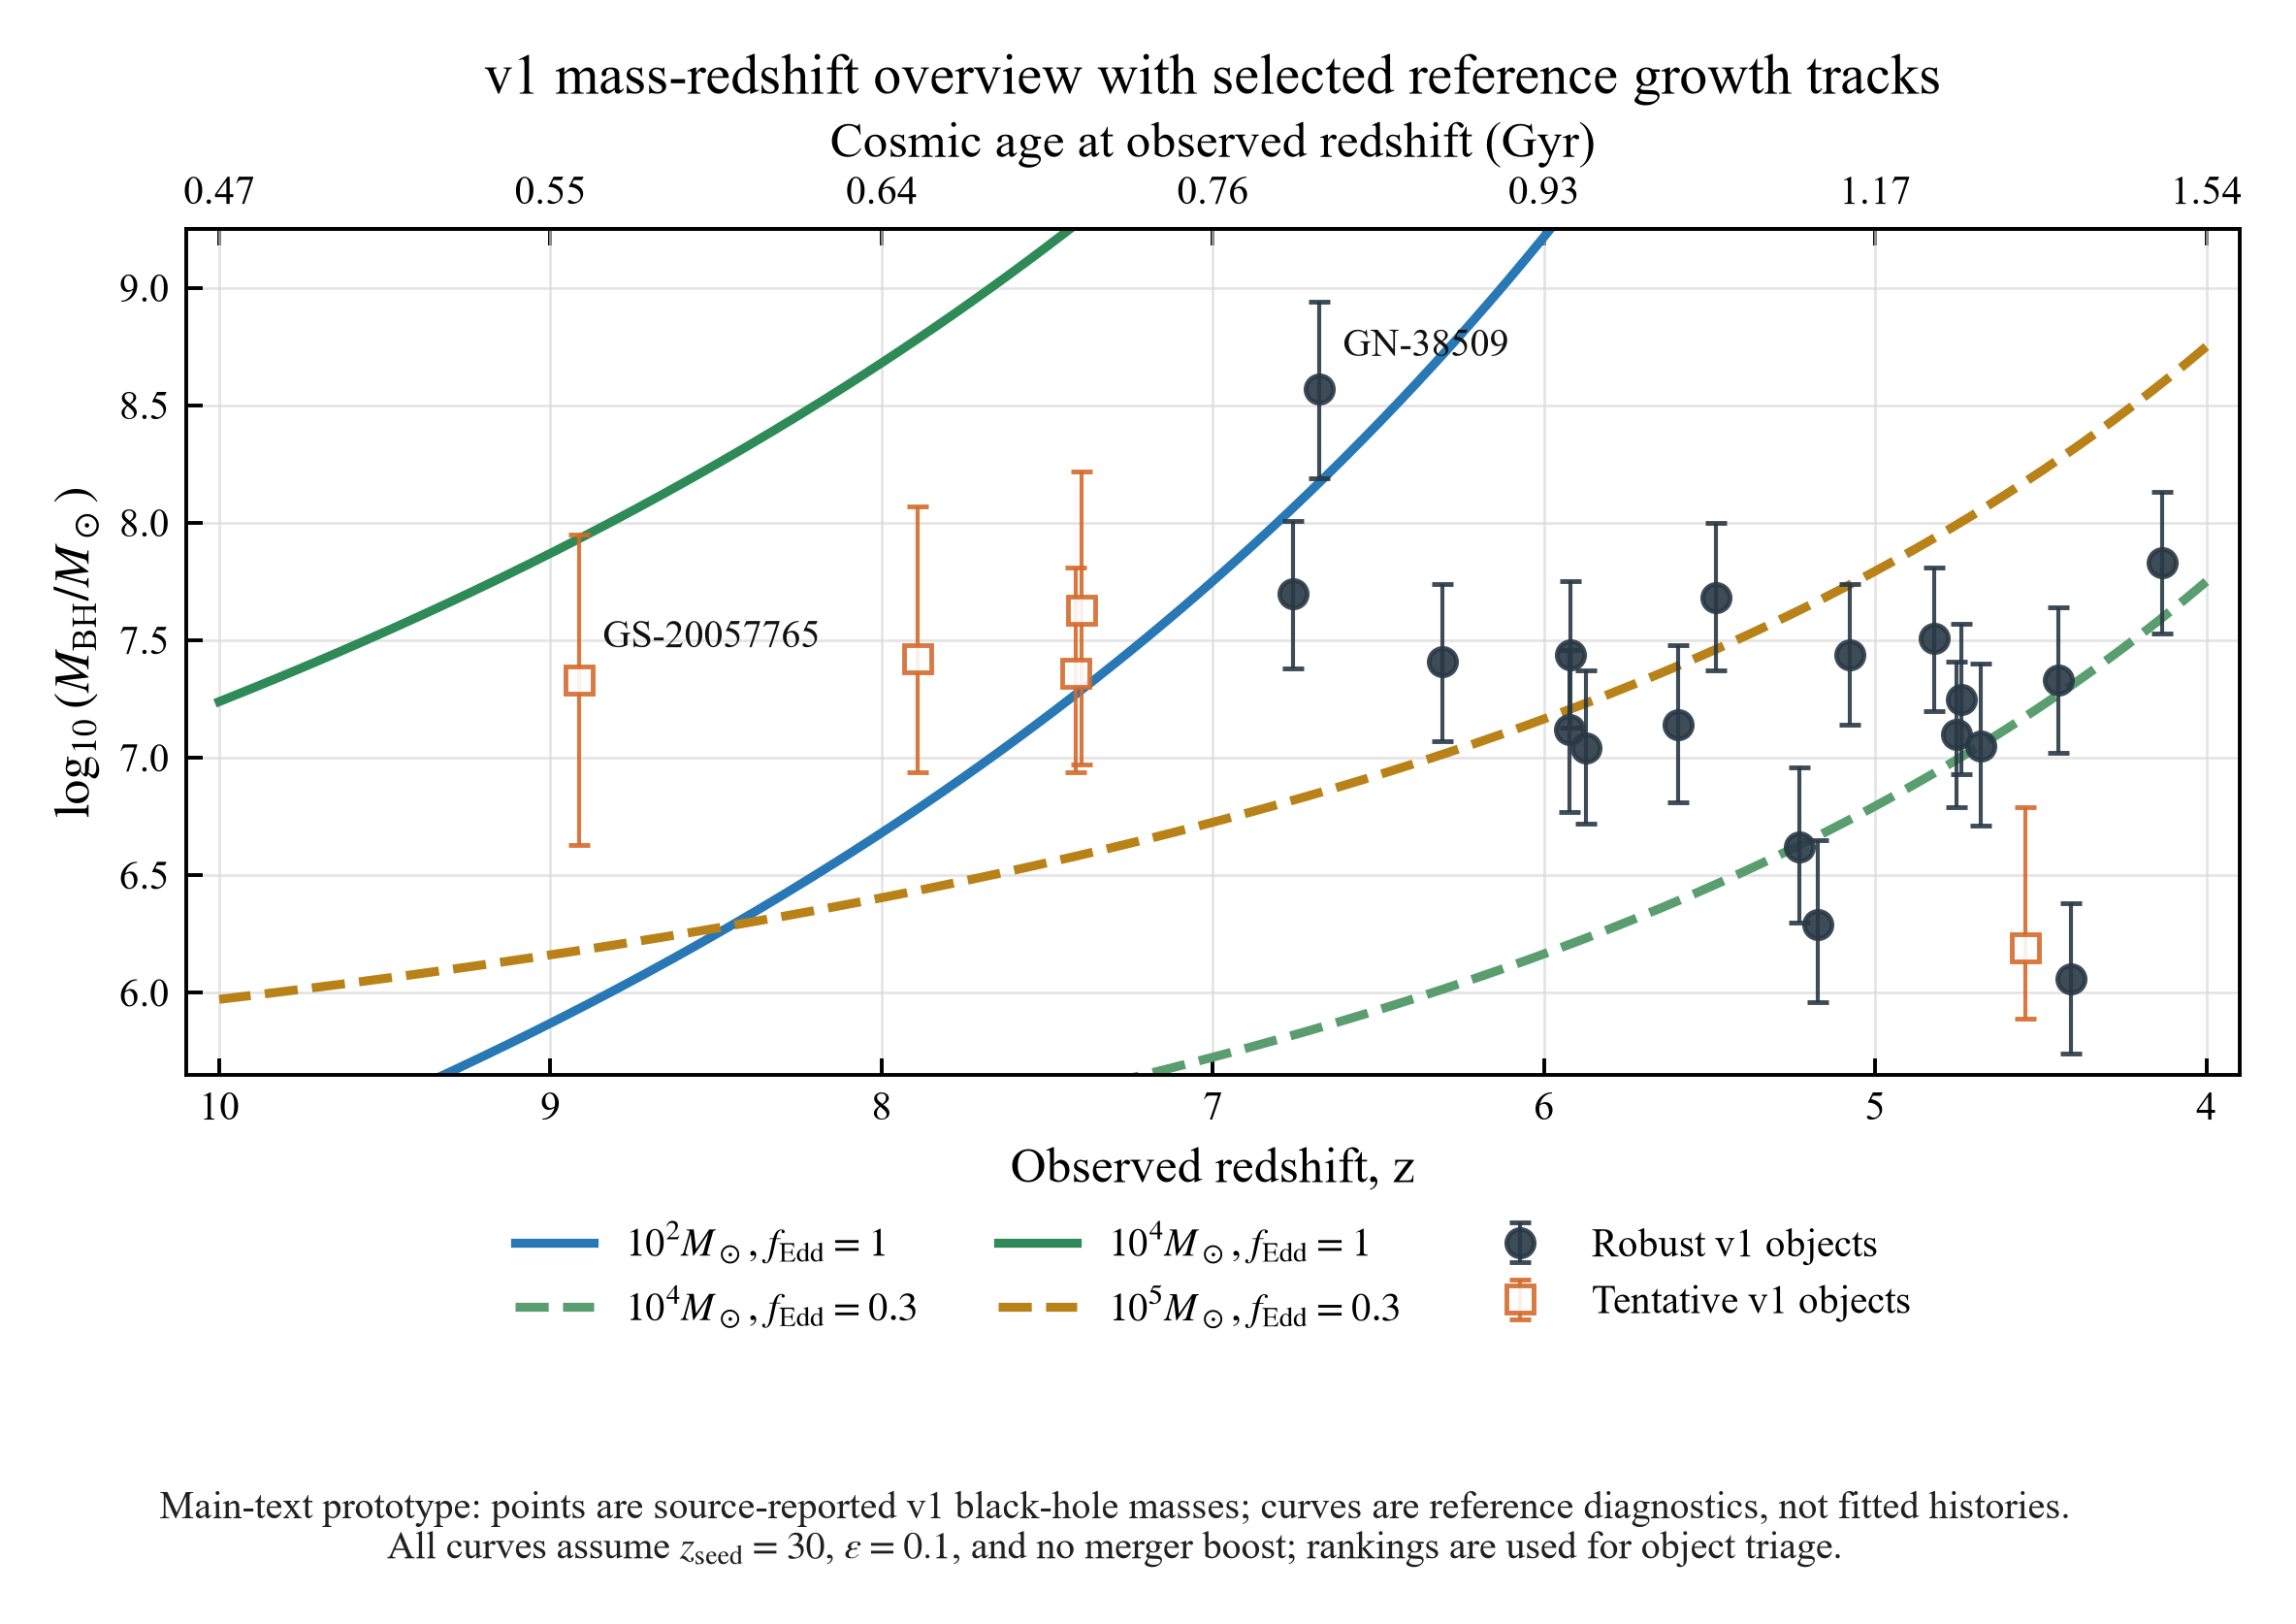
\includegraphics[width=0.91\textwidth]{../results/v2_main_text_figures/v2_main_text_mbh_redshift_growth_overview.png}
\caption{The v1 JADES broad-line AGN sample in black-hole-mass--redshift space. The curves are selected reference growth histories, not fits to the observations. This overview establishes the timing problem before the model is inverted into required-$\fedd$ and required-seed diagnostics.}
\label{fig:overview}
\end{figure}

\subsection{Stage 3 (v2): from scenario grids to observational triage}

The first evaluation stage generated growth tracks, fixed-scenario compatibility summaries, and per-object maps. These products show where each measurement lies across seed mass, accretion, efficiency, merger, and formation-redshift space. They also revealed an important interpretive distinction: a fixed scenario can miss an object through \emph{undergrowth} or \emph{overgrowth}. Only the former directly signals insufficient growth; the latter can be resolved by less accretion, a smaller seed, or later formation.

The project therefore moved from generic compatibility scores to required-parameter rankings. The baseline ranking uses $z_{\rm seed}=30$, $\epsilon=0.1$, and $B_{\rm merge}=1$, and keeps three concepts separate:

\begin{enumerate}
  \item \textbf{Physical pressure:} required $\fedd$ for fixed seeds and required seed mass for fixed accretion histories.
  \item \textbf{Measurement evidence:} detection confidence is recorded separately from line-model and mass-measurement reliability; missing diagnostics are availability metadata rather than automatic penalties.
  \item \textbf{Follow-up value:} the potential for a better measurement to change the physical ranking.
\end{enumerate}

This produces a measurement-level table rather than a single opaque score. Host-mass tension, growth pressure, confidence, and follow-up priority remain independently inspectable.

\subsection{Stage 4: uncertainty propagation}

Point estimates are insufficient near physically meaningful thresholds. The uncertainty layer draws 10,000 samples per measurement from the project's equal-side two-piece normal approximation to the reported asymmetric $\log_{10}\mbh$ uncertainty. The sign of a standard-normal draw selects the reported upper or lower scale, giving each side 50\% probability; this is not the normalized split-normal distribution or a reconstruction of the source posterior. For every draw, the pipeline recomputes the required $\fedd$ and required seed mass. It reports the 5th, 16th, 50th, 84th, and 95th percentiles, together with threshold probabilities.

Three systematic mass scenarios are evaluated separately:
\begin{equation}
\mathrm{baseline},\qquad \log_{10}\mbh-0.3\ \mathrm{dex},\qquad
\log_{10}\mbh+0.3\ \mathrm{dex}.
\end{equation}
The statistical mass sampling is never blended across these systematic scenarios. This separation makes it possible to distinguish reported statistical uncertainty from an assumed method-scale shift.

\subsection{Stage 5 (v3): source expansion and physical-object identity}

The v3 release adds the complete 63-row Table~1 extraction from Taylor et al.\ (2025)~\cite{taylor2025} as a source-specific raw table, then applies $z\geq4$ in the processing layer. The retained Taylor subset has 37 measurements of 36 physical objects, including 17 sources marked as little red dots (LRDs). LRD is stored as a phenotype; the object class remains broad-line AGN. The combined release therefore contains 60 measurements of 59 physical objects.

Every Taylor row preserves coordinates, redshift, total/narrow/broad H$\alpha$ fluxes and uncertainties, broad-line FWHM, formal virial-mass uncertainty, LRD and absorption-fit markers, field/program, and source caveats. The Reines et al.\ (2013) H$\alpha$ single-epoch calibration is tagged precisely, and its approximate $\pm0.5$ dex virial systematic is evaluated separately from formal errors and the common $\pm0.3$ dex comparison. Host mass, bolometric luminosity, and Eddington ratio remain unavailable rather than inferred from absent Table~1 values.

The measurement view retains both CEERS-2782 and RUBIES-EGS-50052. A separate crossmatch maps them to one stable physical-object ID; the higher-S/N RUBIES observation is the documented default for object-level ranking. No measurement is deleted or averaged. Summary tables are stratified by source, survey/field, LRD phenotype, and catalogue view, and mixed-selection rows are marked descriptive rather than demographic.

\subsection{Stage 6 (v4): generalized identity and complementary WFSS samples}

The v4 release adds all 20 Matthee et al.\ EIGER/FRESCO broad-H$\alpha$ emitters~\cite{matthee2024} and all 16 Lin et al.\ ASPIRE emitters~\cite{lin2024} from authoritative arXiv source archives. Both papers use the Reines et al.\ (2013) H$\alpha$ single-epoch estimator and state a 0.5 dex calibration or intrinsic uncertainty. Native line luminosities, widths, photometry, continuum slopes, formal errors, LRD labels, absorption-fit flags, and row caveats are retained. Source-reported host mass and Eddington ratio remain missing; H$\alpha$-derived bolometric luminosities are retained where published.

The identity layer performs deterministic coordinate/redshift candidate searches against both the prior release and other newly added sources, refuses ambiguous matches, and requires an explicit accepted/rejected decision in a reviewed override registry. Review confirms one new cross-paper identity: Matthee GOODS-S-13971 is JADES GS-204851 at 0.02 arcsec separation and $\Delta z=0.001$. The prior-release JADES measurement remains the default for longitudinal reproducibility, while the Matthee row remains independently rankable. Together with the Taylor pair, v4 contains 96 measurements but 94 physical objects.

The v4 science workflow preserves the baseline assumptions and reported asymmetric errors, keeps the common $\pm0.3$ dex comparisons, and adds separately named $\pm0.5$ dex Reines-calibration scenarios for Taylor, Matthee, and ASPIRE. Detection confidence is now distinct from mass/line-model reliability, so robust broad-line detections with absorption or contamination caveats receive caveated follow-up categories without being relabelled as tentative detections. Object-level LRD unions retain supporting measurement and source provenance. Overall summaries explicitly mix unlike selection functions and are descriptive only.

The v4.0.1 method registry also resolves a previously implicit JADES distinction. The 19 H$\alpha$ measurements use the Reines \& Volonteri (2015) relation and the source paper states a 0.3 dex calibration uncertainty. The four tentative H$\beta$ measurements use Vestergaard \& Peterson (2006); because the JADES paper does not assign that estimator a numeric systematic, the registry leaves it unavailable and retains the paper's $A_V=0$ underestimation caveat. These metadata are not folded into the reported statistical errors and do not retroactively alter the frozen v4 scenarios.

\subsection{Stage 7 (v5): Harikane measurement version and taxonomy foundation}

v5 ingests all ten final-sample Type 1 broad-H$\alpha$ measurements from Harikane et al.\ (2023)~\cite{harikane2023}. Five rows match existing CEERS physical objects and five create new stable objects, producing 106 measurements and 99 physical objects. CEERS-02782 becomes a third retained measurement of the CEERS-2782/RUBIES-EGS-50052 object; the established RUBIES default remains unchanged. Four published host-mass upper limits remain limits rather than canonical measurements, and the absent row-level LRD designation remains missing rather than being inferred from red or compact phenotypes.

Harikane masses use the Greene \& Ho (2005) H$\alpha$ single-epoch relation applied to extinction-corrected broad-H$\alpha$ luminosity. The paper supplies asymmetric statistical errors but no numeric virial-calibration systematic, so v5 propagates the reported errors and applies only the common $\pm0.3$ dex comparison scenarios to these rows. The source-specific Taylor, Matthee, and ASPIRE $\pm0.5$ dex sensitivities remain separate. Orthogonal taxonomy fields now distinguish evidence strength, spectroscopic type, selection channel, phenotype, lensing status, and growth-ranking eligibility while every current row remains a broad-line AGN.

\subsection{Stage 8 (v6): Davis/THRILS final same-class consolidation}

The v6 source gate verified the complete seven-row broad-H$\alpha$ Appendix Table 5 of Davis et al.\ (2026)~\cite{davis2026}. Processing retains six rows at $z\geq4$; the sole below-cut THRILS row is a known Taylor repeat and remains in immutable raw history. Coordinates and more precise programme redshifts are joined exactly by THRILS ID from the primary THRILS programme catalogue~\cite{hutchison2025}. None of the six retained rows matches a v5 object within the fixed coordinate/redshift thresholds, so v6 contains 112 measurements and 105 physical objects.

Davis masses use the Reines \& Volonteri (2015) H$\alpha$ single-epoch relation. Formal posterior errors remain statistical, while the source's approximately 0.5 dex recipe scatter is represented only by separately labelled sensitivity scenarios. Table 5 does not publish row-level LRD, host mass, bolometric luminosity, or Eddington ratio, and only THRILS 40467 has a source-text FWHM; missing values are not reconstructed. The highest-pressure new object is THRILS 25501 at point primary rank 23 and uncertainty primary rank 36, so the established leading objects remain unchanged. This extends coverage without supporting a pooled demographic claim.

\begin{figure}[p]
\centering
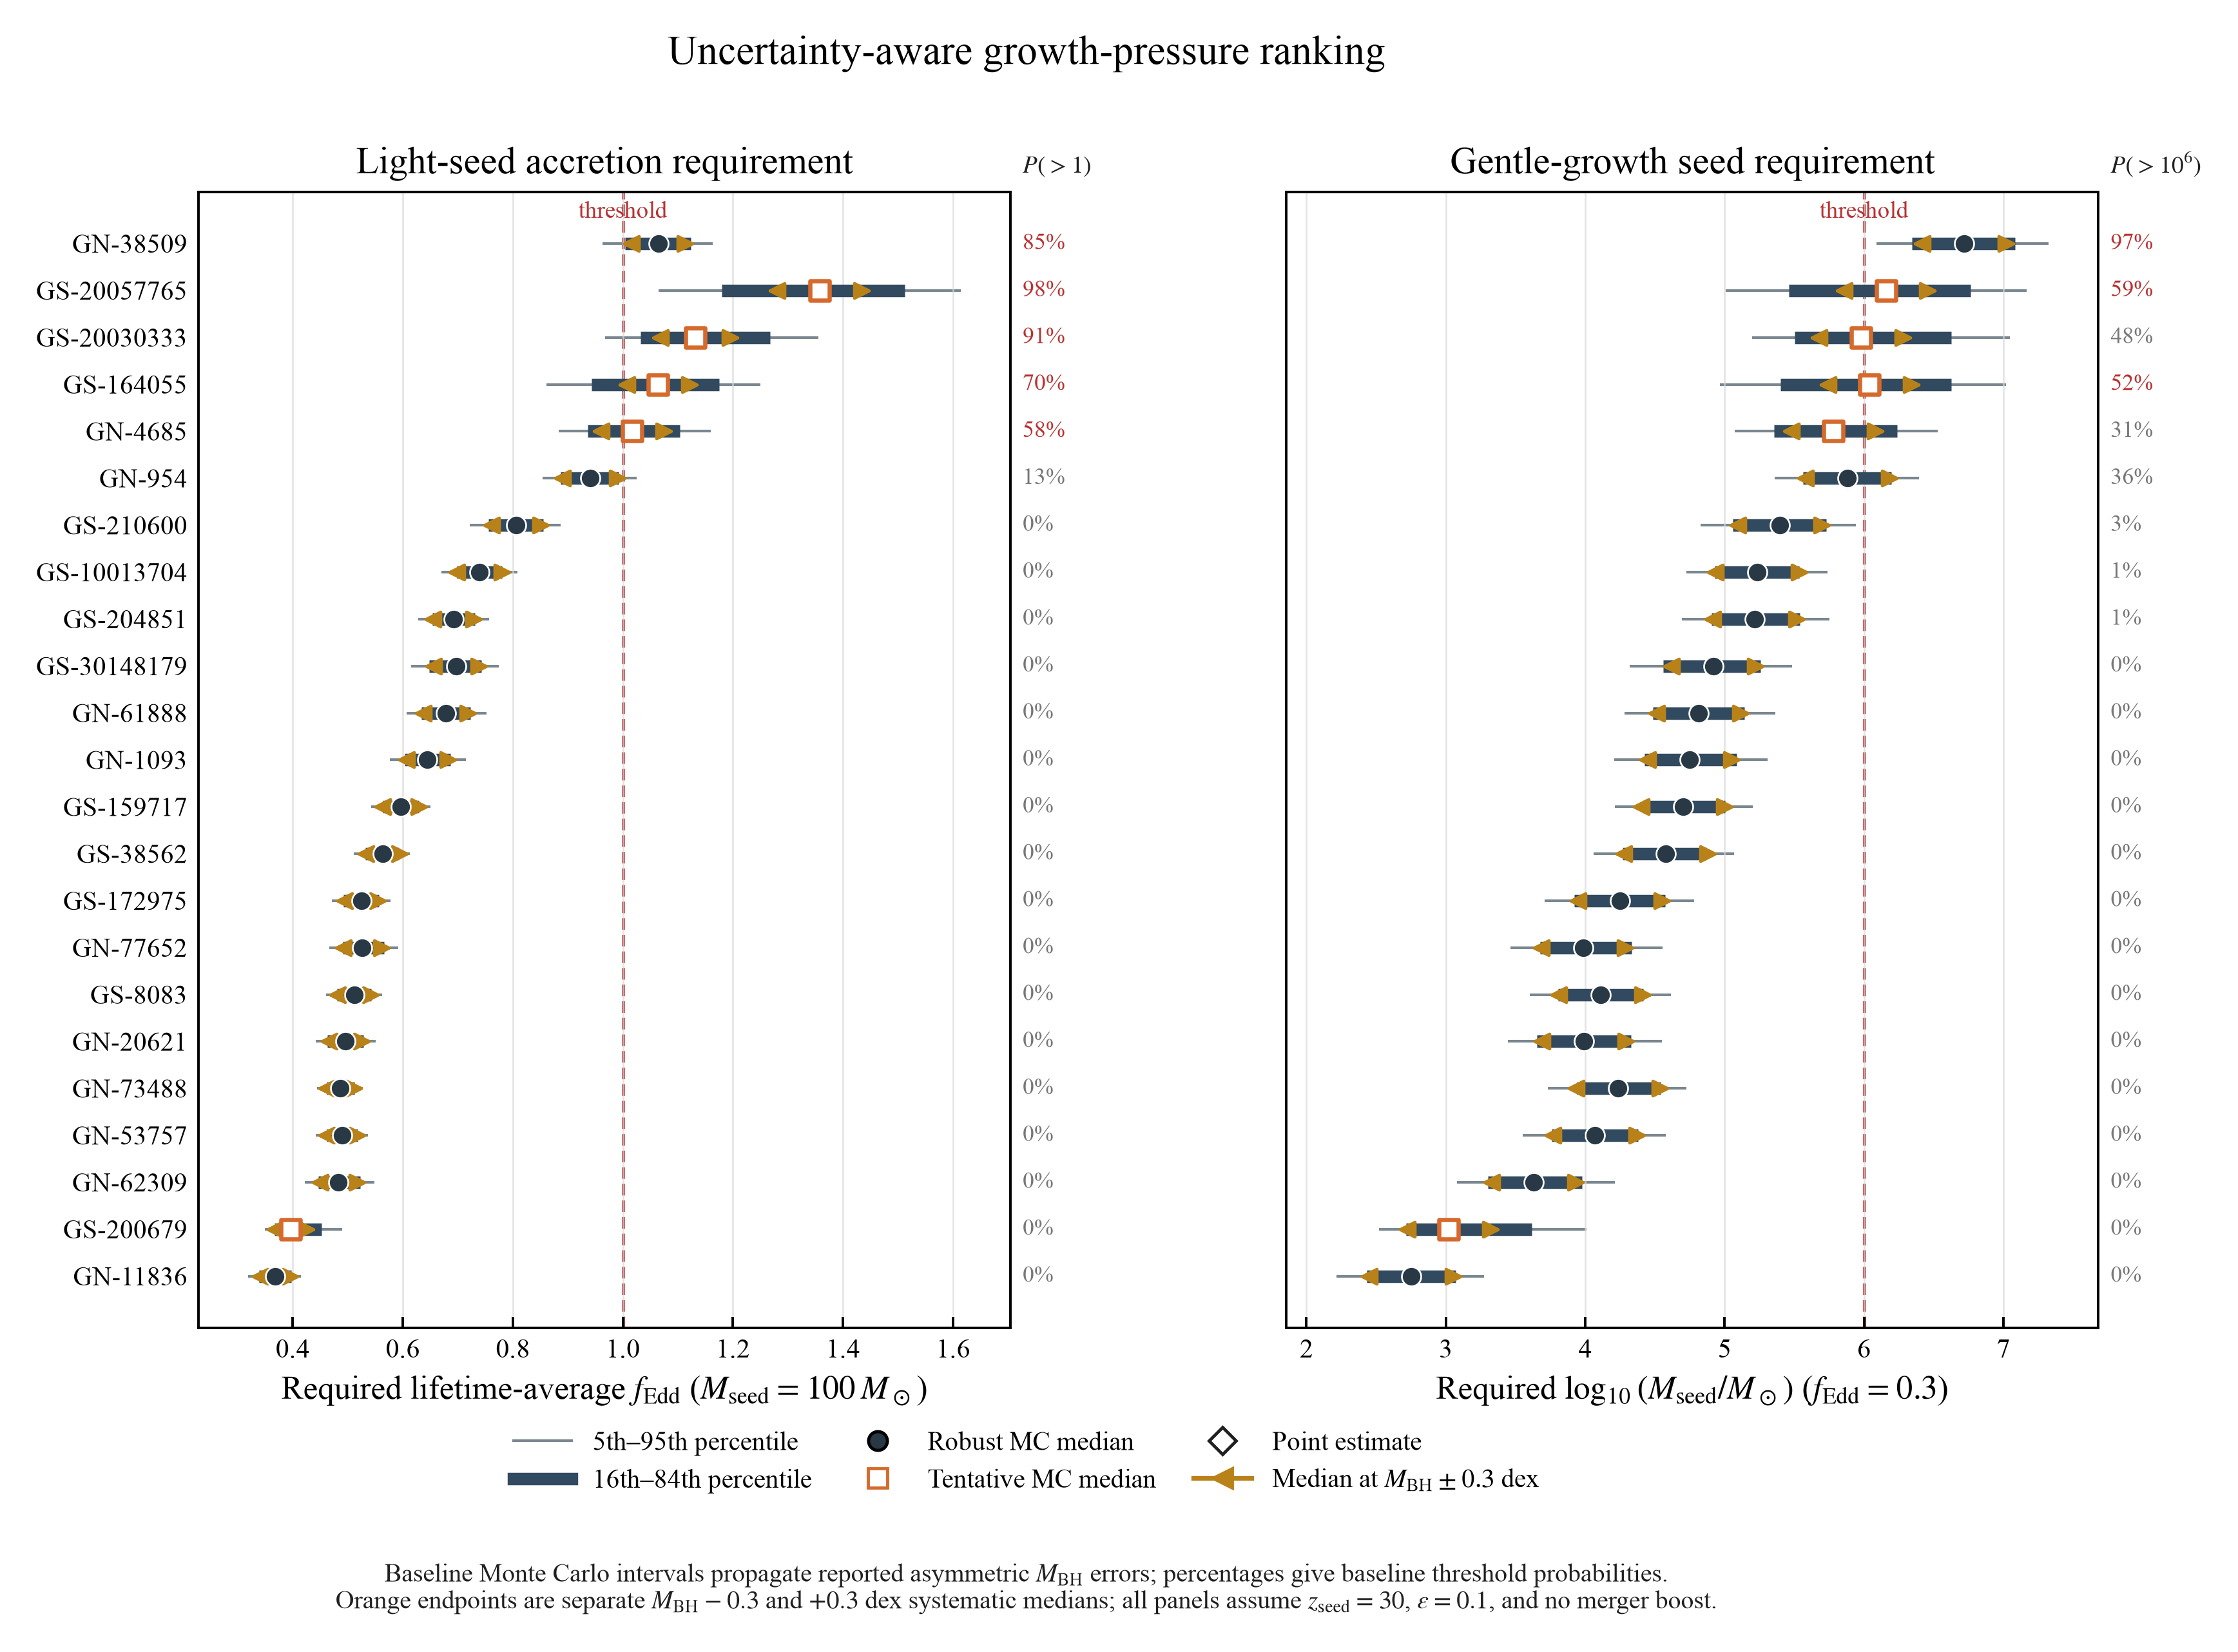
\includegraphics[width=0.99\textwidth]{../results/v2_main_text_figures/v2_main_text_uncertainty_forest.png}
\caption{Uncertainty-aware growth-pressure ranking. Thin and thick intervals show the baseline 5th--95th and 16th--84th percentiles. Circles and open squares denote robust and tentative Monte Carlo medians; diamonds are the original point estimates. Orange endpoints show the separate $\mbh\pm0.3$ dex systematic medians. Red dashed lines mark $\fedd=1$ for a $100\,M_\odot$ seed (left) and $\mseed=10^6\,M_\odot$ for $\fedd=0.3$ (right). Percentages give baseline probabilities of crossing the corresponding threshold.}
\label{fig:uncertainty}
\end{figure}

\begin{figure}[p]
\centering
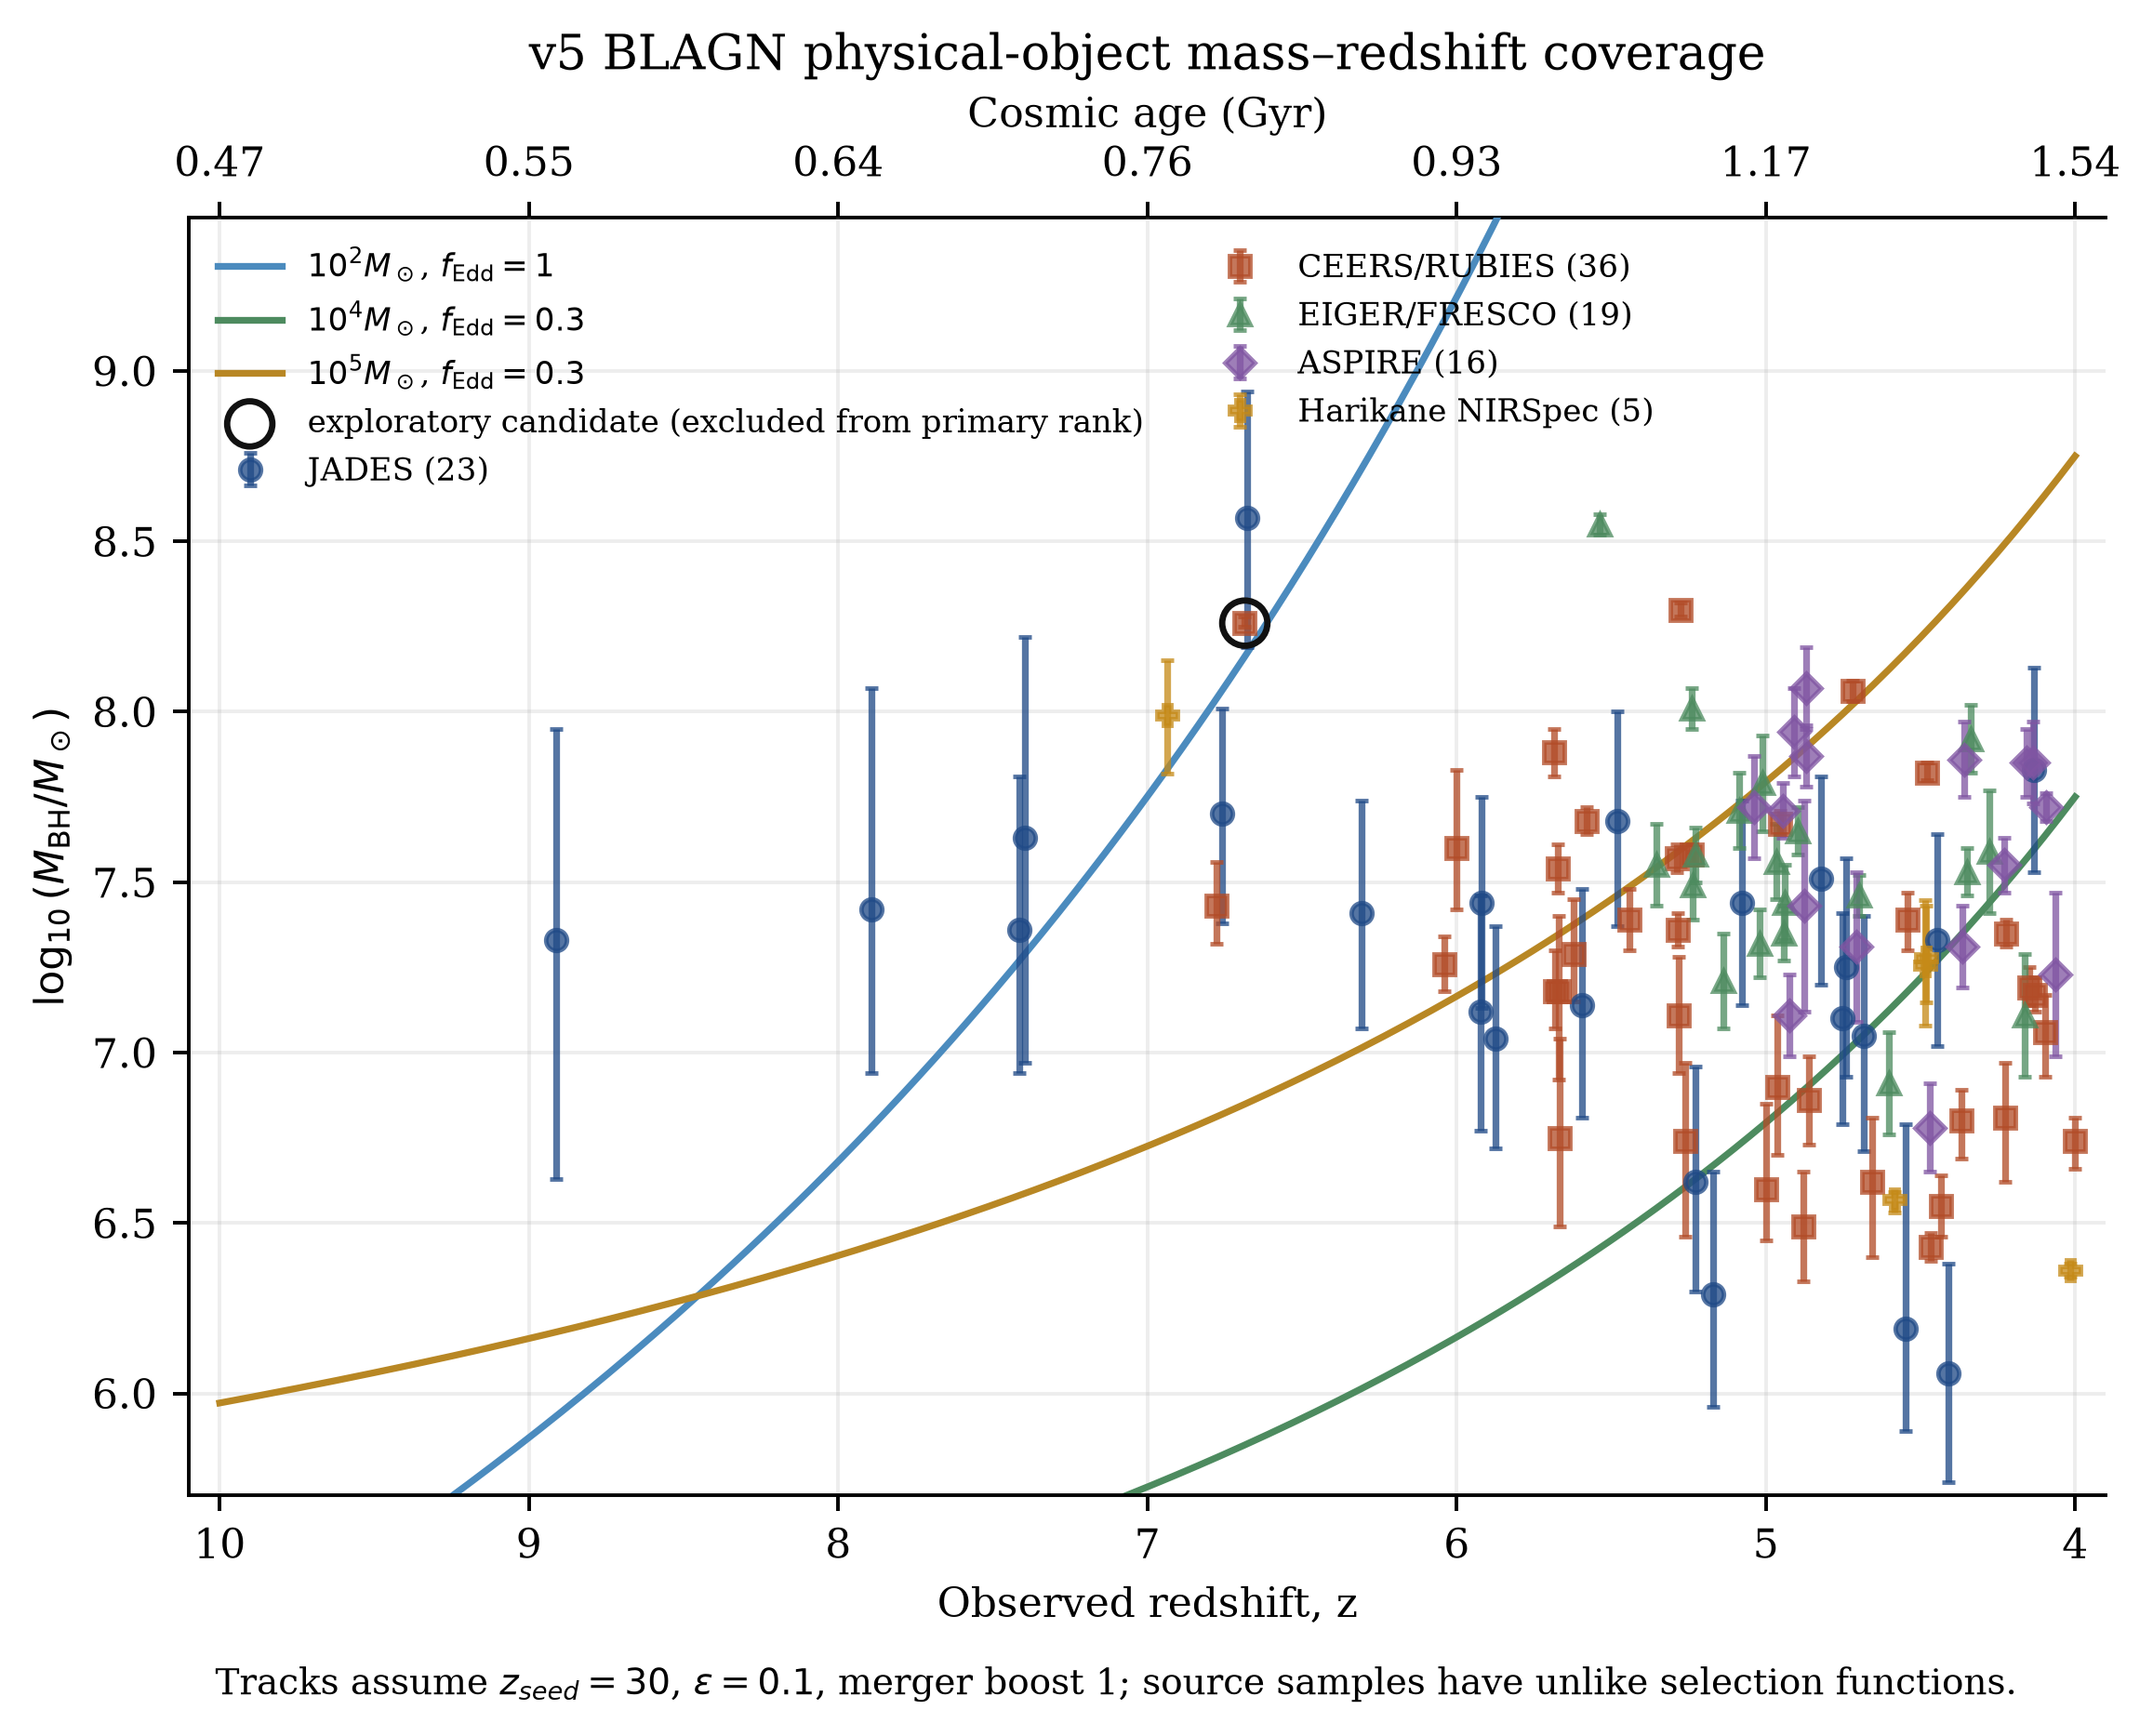
\includegraphics[width=0.94\textwidth]{../results/v5_main_text_figures/v5_main_text_mbh_redshift_growth_overview.png}
\caption{Latest deliberate rendered overview (v5), stratified across five preferred-measurement source selections. v6 adds six THRILS objects in tables but does not silently regenerate this figure. The open marker identifies the retained alternative-interpretation candidate excluded from the primary rank.}
\label{fig:v4overview}
\end{figure}

\section{Current scientific findings}

The v2 v1-catalogue analysis identifies a stable high-leverage group, but the uncertainty analysis changes how strongly individual objects should be described. The v3 object-level ranking retains GN-38509 and GS-20057765 in the first two positions and adds RUBIES-EGS-49140 in third; the Taylor object is flagged for possible outflow contribution or an alternative non-AGN broad-line interpretation. Table~\ref{tab:objects} retains the detailed v1 probabilities that underlie the first comparison.

\begin{table}[ht]
\centering
\caption{Primary evidence-supported v6 physical-object growth-pressure leaders under the baseline reference. The leading five are unchanged from v5; the complete diagnostic ordering is retained separately and is exploratory.}
\label{tab:v5leaders}
\small
\begin{tabular}{@{}lclrr@{}}
\toprule
Primary rank & Object & Preferred source & $f_{\rm Edd,req}^{100}$ & $\log M_{\rm seed,req}^{0.3}$ \\
\midrule
1 & GN-38509 & JADES & 1.065 & 6.719 \\
2 & GS-20057765 & JADES & 1.355 & 6.150 \\
3 & CEERS-00717 & Harikane & 1.027 & 6.242 \\
4 & GOODS-N-9771 & Matthee & 0.810 & 6.124 \\
5 & GS-164055 & JADES & 1.065 & 6.044 \\
\bottomrule
\end{tabular}
\end{table}

The complete 105-object diagnostic ordering is deliberately exploratory: its first three entries are GN-38509, GS-20057765, and RUBIES-EGS-49140, but the last object is an alternative-interpretation candidate and therefore has no primary rank. In the 104-object primary uncertainty ordering, GN-38509 and GS-20057765 remain first and second, GOODS-N-9771 is third, CEERS-00717 is fourth, and GS-20030333 is fifth. The highest THRILS object, THRILS 25501, enters point primary rank 23 and uncertainty primary rank 36. Point and uncertainty rank answer related but distinct questions; neither is a population-frequency statement.

\begin{table}[ht]
\centering
\caption{Highest-leverage v1 measurements under the baseline uncertainty model.}
\label{tab:objects}
\small
\begin{tabular}{@{}lcccl@{}}
\toprule
Object & Quality & $P(f_{\rm Edd,req}^{100}>1)$ & $P(M_{\rm seed,req}^{0.3}>10^6M_\odot)$ & Status \\
\midrule
GN-38509 & robust & 0.85 & 0.97 & strongest robust pressure case \\
GS-20057765 & tentative & 0.98 & 0.59 & strongest tentative follow-up target \\
GS-20030333 & tentative & 0.91 & 0.48 & high leverage; elevated BH/host ratio \\
GS-164055 & tentative & 0.70 & 0.52 & high leverage; extreme BH/host ratio \\
GN-4685 & tentative & 0.58 & 0.31 & threshold and systematics sensitive \\
GN-954 & robust & 0.13 & 0.36 & comparison/systematics object \\
\bottomrule
\end{tabular}
\end{table}

GN-38509 is currently the clearest robust result: it remains demanding in both light-seed and gentle-growth diagnostics after propagating the reported mass uncertainty. GS-20057765 is more extreme in the light-seed calculation but is tentative and has a broader required-seed distribution. It is therefore a high-priority follow-up target rather than an equally secure theoretical constraint. GN-954 illustrates why probability statements matter: its point estimate is near a pressure boundary, but its baseline probability of requiring super-Eddington lifetime-average growth from a $100\,M_\odot$ seed is only 0.13.

The reported Eddington ratios are instantaneous observational estimates, whereas the model-derived $\fedd$ values are lifetime averages. The v5 extension now evaluates the effective two-state relation $\langle\fedd\rangle=D f_{\rm Edd,burst}+(1-D)f_{\rm Edd,quiet}$ with $f_{\rm Edd,quiet}=0$ and $f_{\rm Edd,burst}=1,2,3$. For the 99 object defaults, the median required duty cycles are 0.574, 0.287, and 0.191, respectively. Seven objects exceed $D=1$ in the $f_{\rm Edd,burst}=1$ point scenario (six in the primary population); none do so for burst rates 2 or 3. These are fixed-assumption feasibility diagnostics, not reconstructed light curves, and the 28 published current object-level ratios are not substituted for historical averages. A separate source-table cross-check identifies GN-11836 as internally inconsistent: its published $\log M_{\rm BH}=6.06$ and $\log L_{\rm bol}=44.11$ imply $\lambda_{\rm Edd}\simeq0.89$, while the table reports 0.11. All published values are retained pending clarification, but the current-to-required ratio is left missing and the row is explicitly ineligible for that comparison.

\begin{figure}[p]
\centering
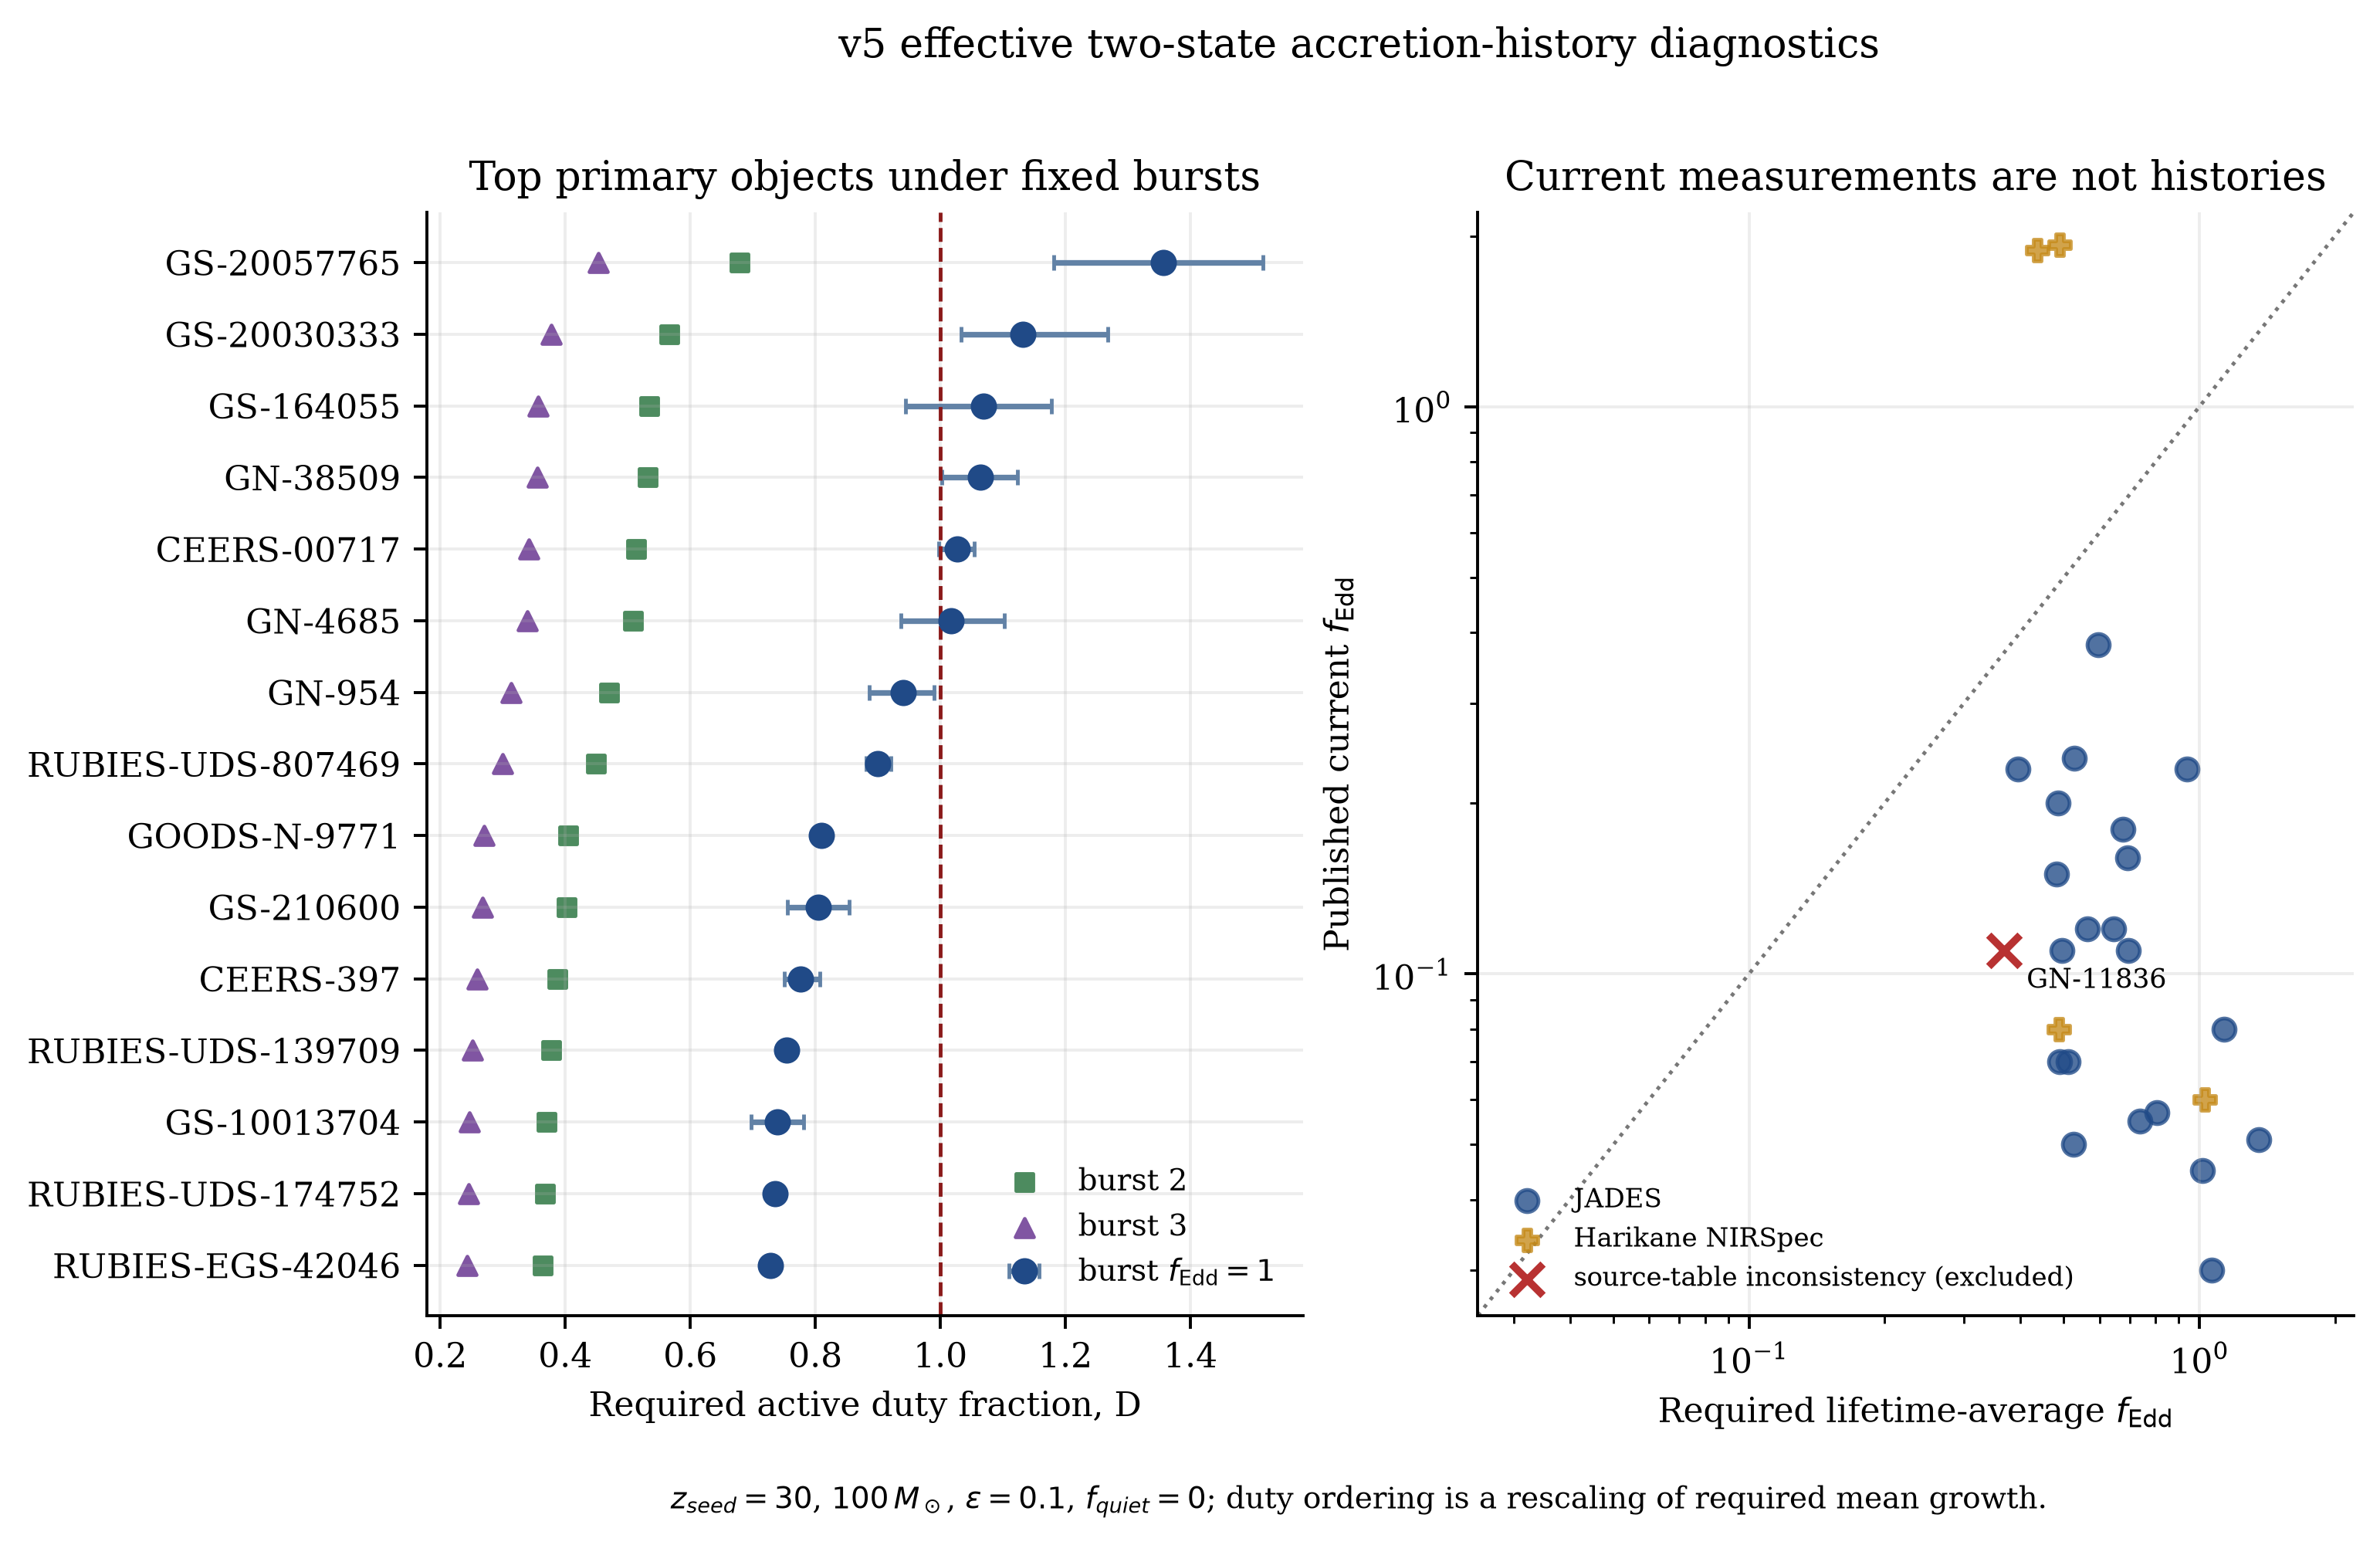
\includegraphics[width=0.98\textwidth]{../results/v5_main_text_figures/v5_main_text_accretion_history_diagnostics.png}
\caption{Current v5 effective two-state diagnostics. The left panel shows required duty fractions for fixed burst rates; because each is a monotonic rescaling of the required lifetime-average rate, the canonical primary growth rank is retained rather than inventing a redundant duty-cycle rank. The right panel keeps published current Eddington ratios distinct from historical requirements and marks GN-11836 as retained but excluded from ratio use.}
\label{fig:v5history}
\end{figure}

The corrected v4 point ranking kept GN-38509 first, GS-20057765 second, and RUBIES-EGS-49140 third. Those three remain the v5 complete exploratory leaders; RUBIES-EGS-49140 has no primary rank because of its alternative interpretation. Harikane CEERS-00717 enters point-estimate growth-pressure rank 4 and uncertainty-aware rank 5, while GOODS-N-9771 shifts from v4 point rank 4 to v5 rank 5. Seven nondefault measurements are now tested one at a time, including the three-measurement CEERS-2782 object. These are sensitivity results, not changes to release defaults.

\begin{figure}[p]
\centering
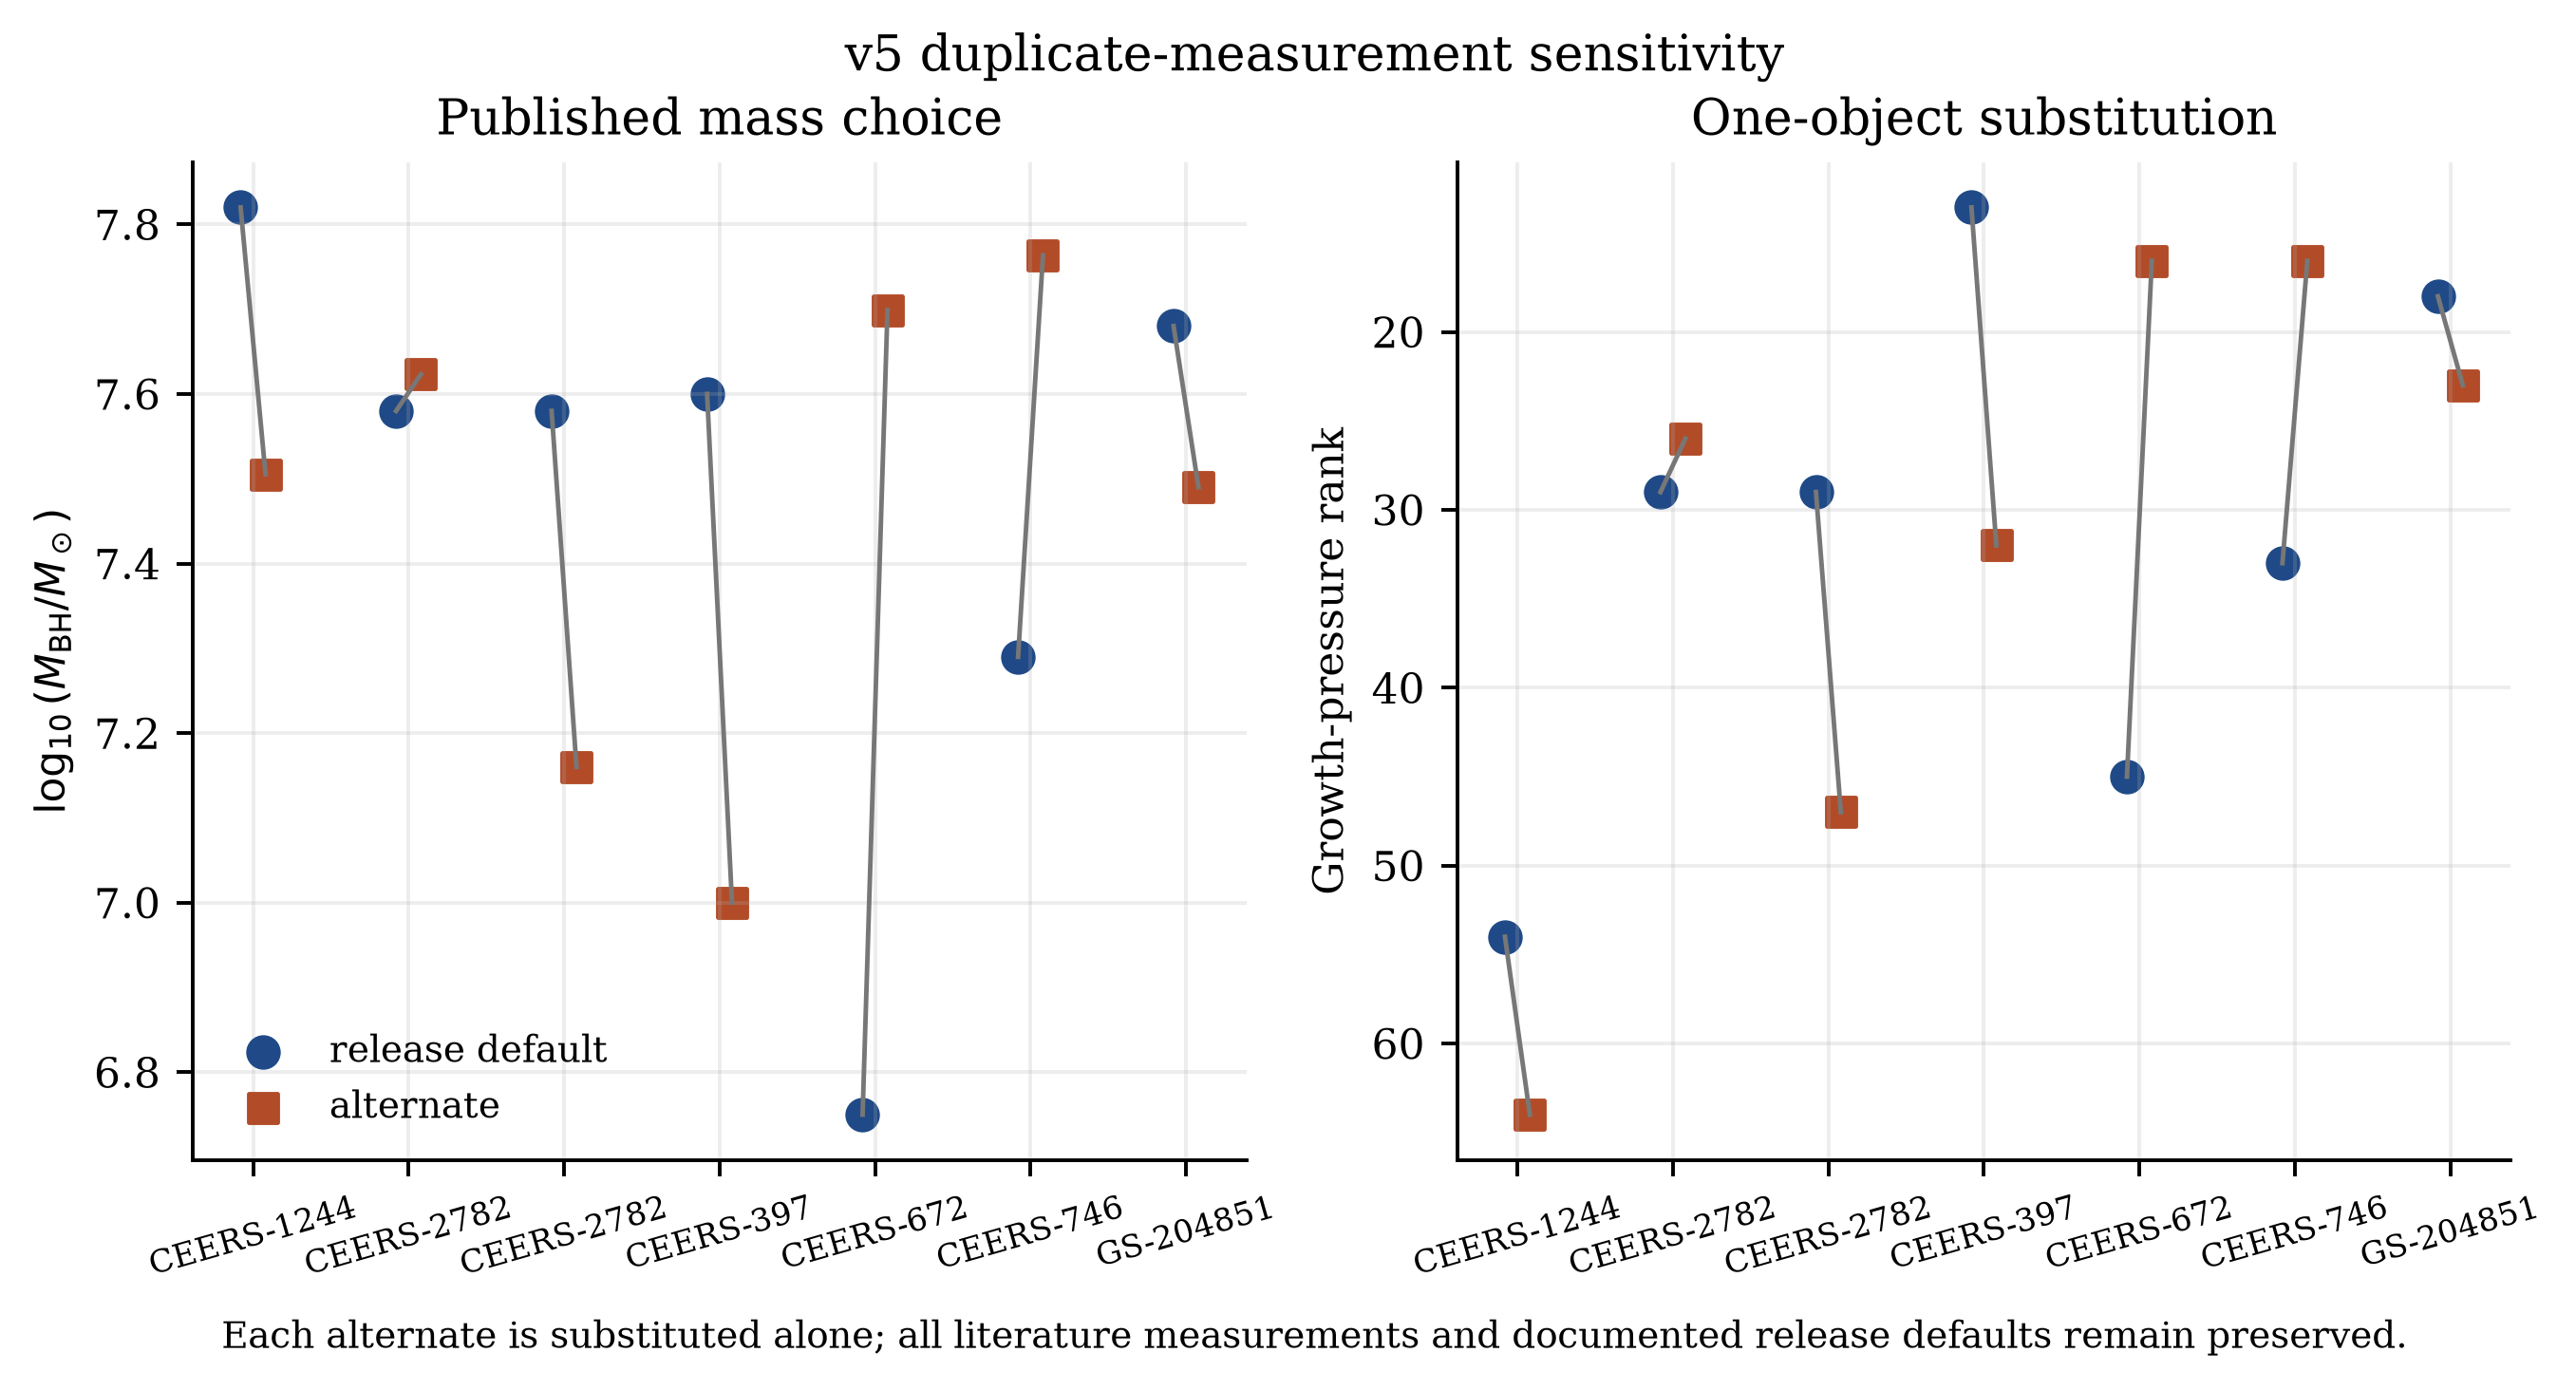
\includegraphics[width=0.94\textwidth]{../results/v5_main_text_figures/v5_appendix_measurement_choice_sensitivity.png}
\caption{Current-v5 one-at-a-time sensitivity to all seven nondefault literature measurements. The exercise recomputes the full 99-object ranking while preserving every published row and documented release default.}
\label{fig:v4measurementchoice}
\end{figure}

\begin{figure}[p]
\centering
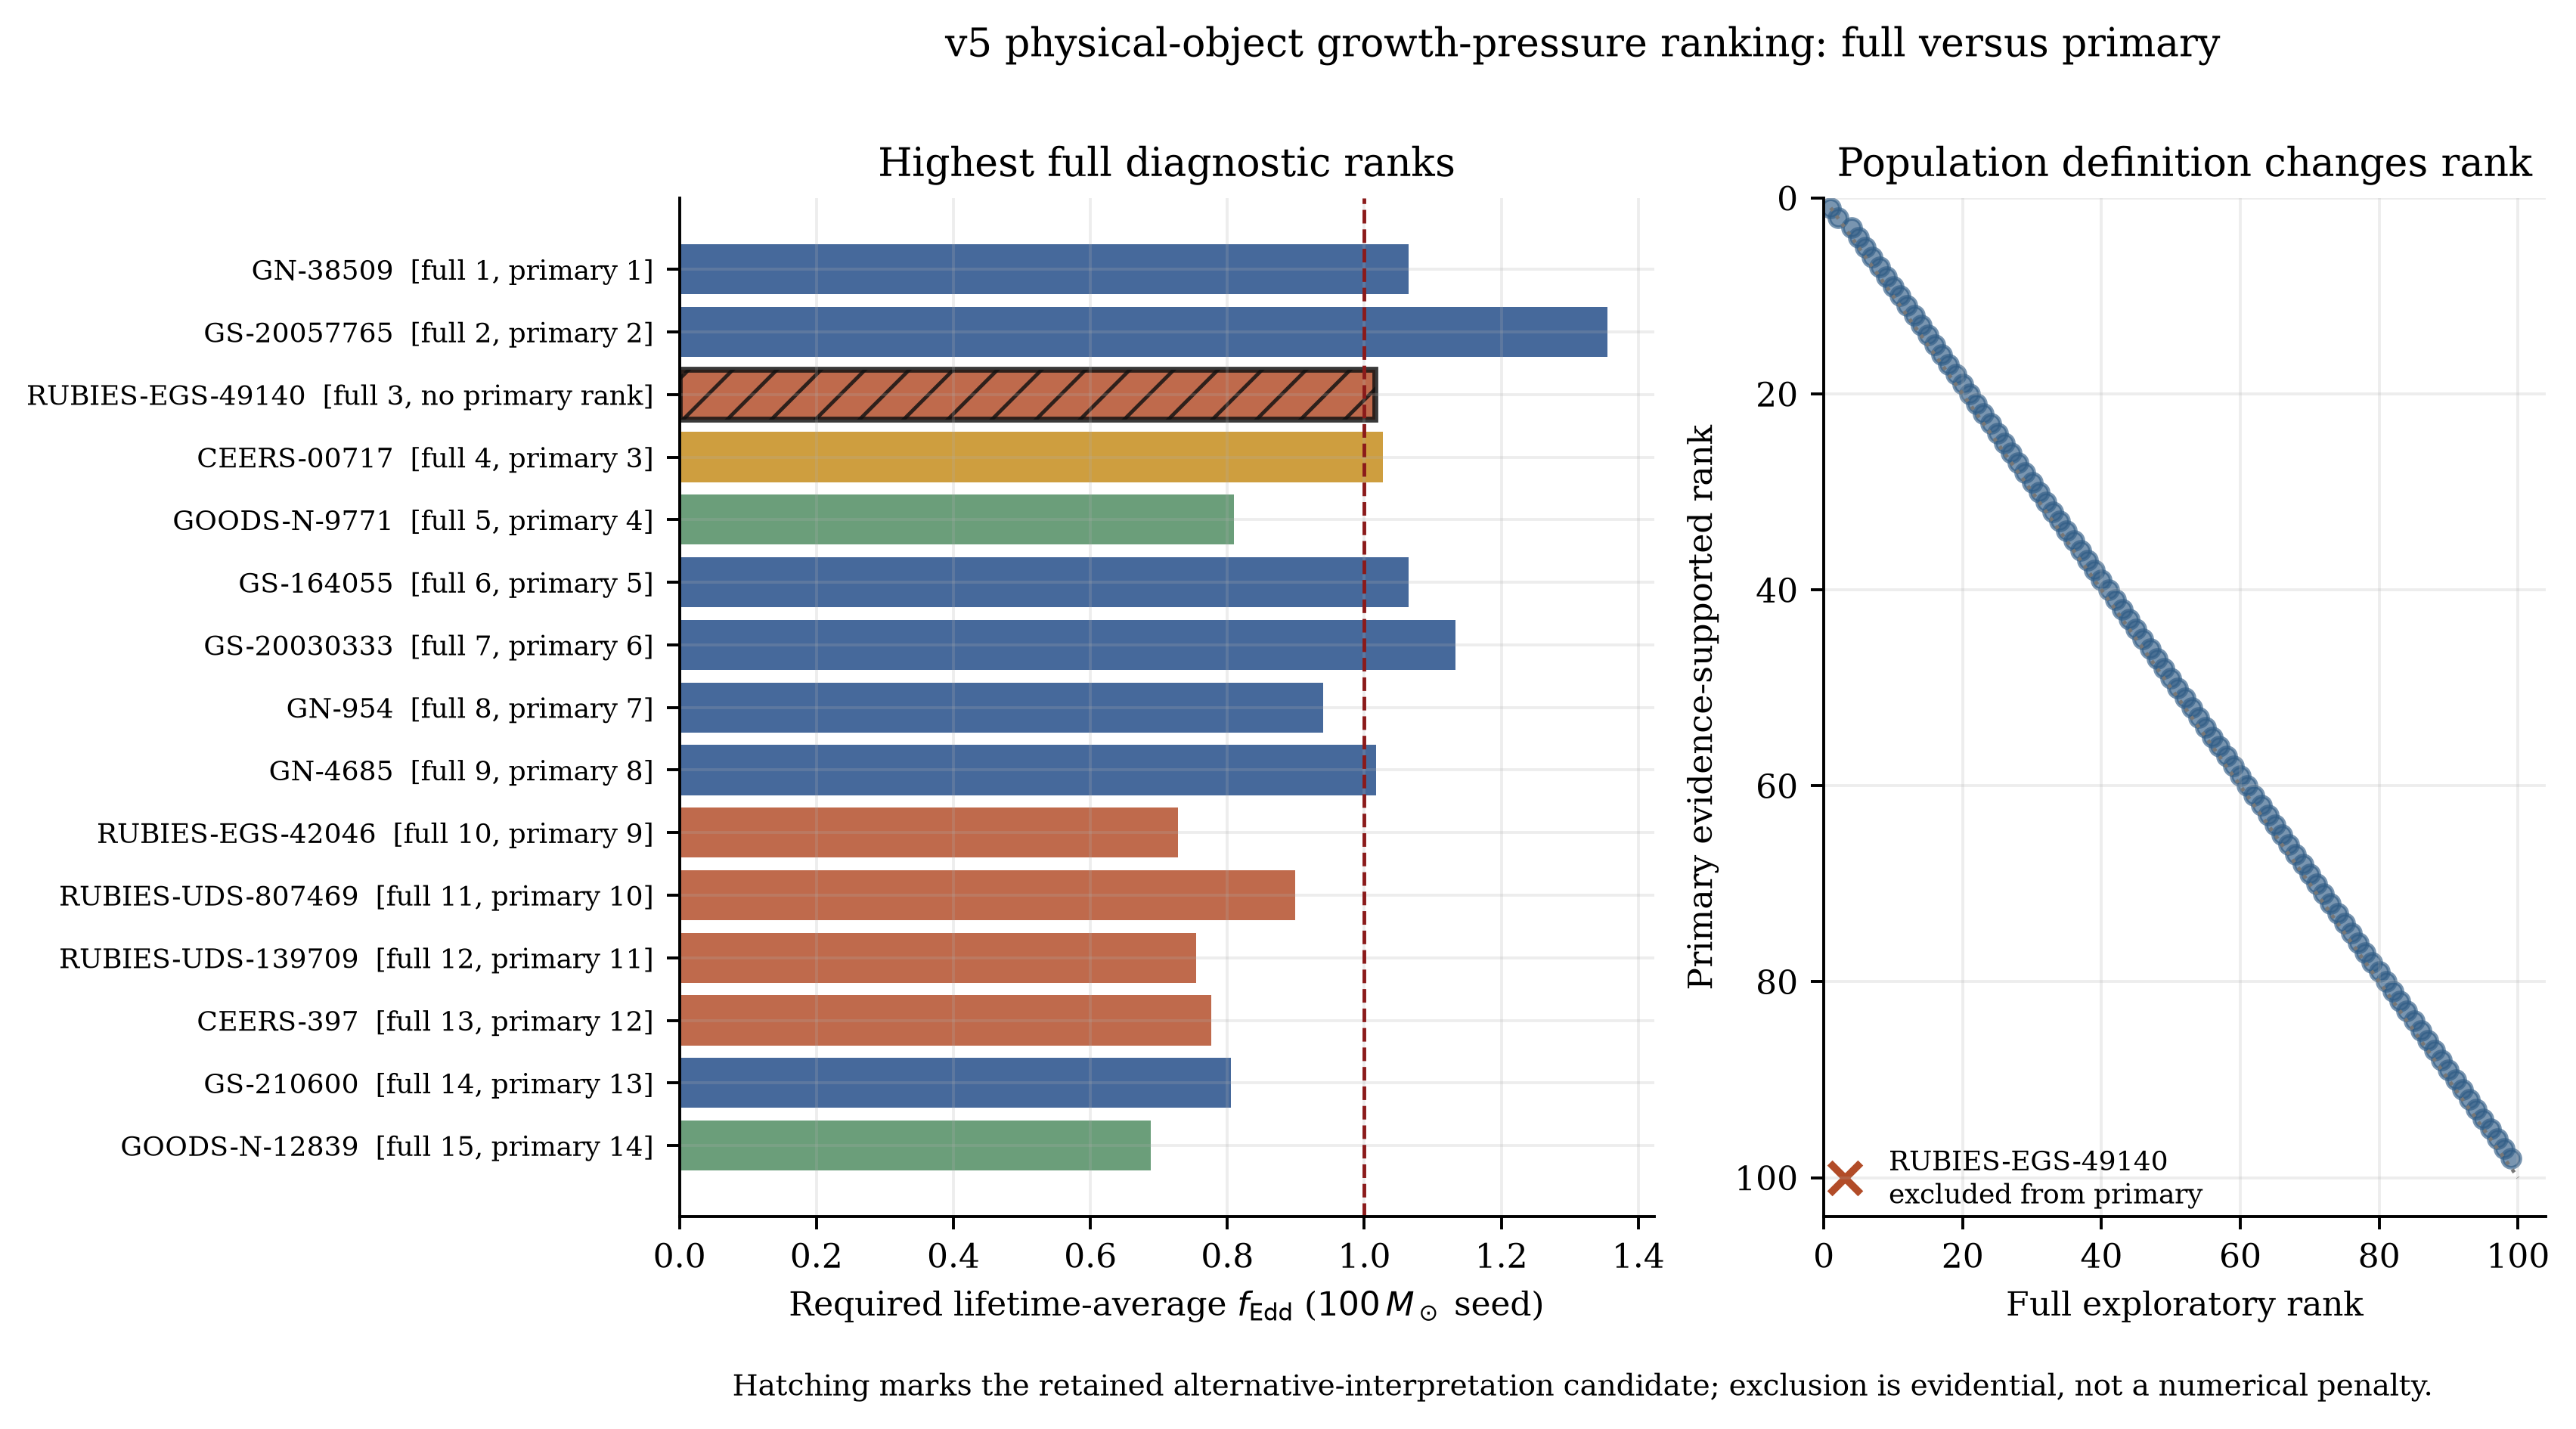
\includegraphics[width=0.98\textwidth]{../results/v5_main_text_figures/v5_main_text_primary_vs_full_ranking.png}
\caption{Current-v5 full versus primary physical-object growth-pressure ranking. The candidate remains visible in the complete diagnostic ordering but receives no evidence-supported primary rank; exclusion is evidential rather than a numerical score penalty.}
\label{fig:triage}
\end{figure}

\section{Release map and reproducibility}

The project versions are chronological milestones: v1 is the pilot JADES catalogue and baseline evaluation, v2 is ranking/uncertainty/figure analysis on that frozen catalogue, v3 is the combined JADES + Taylor catalogue, v4 generalizes identity while adding Matthee and ASPIRE, v5 adds Harikane measurement versions plus taxonomy scaffolding, and v6 completes the same-class foundation with Davis/THRILS. Source-paper versions, including arXiv suffixes, are independent provenance metadata. The canonical dependency map is:

\begin{enumerate}
  \item \repo{data/sources.md} and \repo{data/raw/v1\_raw.csv}: source provenance and extracted measurements.\par
  \item \repo{docs/catalogue-schema.md}: canonical fields, validation rules, and missing-value policy.\par
  \item \repo{src/standardize\_data.py} and \repo{scripts/process\_data.py}: raw-to-processed catalogue construction.\par
  \item \repo{src/models.py}: cosmology and black-hole growth calculations.\par
  \item \repo{src/scoring.py} and \repo{scripts/v1\_evaluate.ipynb}: scenario evaluation and exploratory compatibility products.\par
  \item \repo{scripts/generate\_v2\_rankings.py}: v2 point-estimate physical-pressure and follow-up rankings from v1.\par
  \item \repo{scripts/generate\_v2\_uncertainty\_rankings.py}: v2 deterministic Monte Carlo summaries and probability-based rankings.\par
  \item \repo{scripts/generate\_v2\_final\_figures.py}: v2 publication-style figures driven by the v1-catalogue result tables.\par
  \item \repo{scripts/process\_v3\_blagn.py} and \repo{src/v3\_catalogue.py}: v3 source combination, crossmatch, and object view.\par
  \item \repo{scripts/generate\_v3\_blagn\_science.py} and \repo{src/v3\_science.py}: v3 measurement/object evaluation, rankings, uncertainty, and summaries.\par
  \item \repo{scripts/generate\_v3\_final\_figures.py}: frozen-v3 comparison figures.\par
  \item \repo{scripts/process\_v4\_blagn.py}, \repo{src/identity.py}, and \repo{src/v4\_catalogue.py}: v4 ingestion, pairwise candidate generation, explicit reviewed decisions, aliases, and measurement/object views.\par
  \item \repo{scripts/generate\_v4\_blagn\_science.py} and \repo{src/v4\_science.py}: v4 point and uncertainty products, confidence/reliability separation, phenotype attribution, and duplicate-measurement sensitivity.\par
  \item \repo{requirements-lock.txt}, \repo{releases/v4.0.1-manifest.json}, and \repo{scripts/verify\_v4\_release.py}: exact dependencies, frozen hashes, and write-free in-memory reproduction.\par
  \item \repo{data/mass\_method\_registry.csv}: reviewed source/method calibrations and explicitly unavailable numeric systematics.\par
  \item \repo{scripts/generate\_v4\_final\_figures.py}: the five corrected-v4 figures.\par
  \item \repo{scripts/process\_v5\_blagn.py}, \repo{src/v5\_catalogue.py}, and \repo{src/object\_taxonomy.py}: Harikane ingestion, reviewed identity linkage, and orthogonal taxonomy.\par
  \item \repo{scripts/generate\_v5\_blagn\_science.py} and \repo{src/v5\_science.py}: v5 evaluation, full/primary rankings, uncertainty, summaries, measurement sensitivity, and duty-cycle diagnostics.\par
  \item \repo{scripts/generate\_v5\_final\_figures.py}: the current three main-text and one appendix v5 paper figures.\par
  \item \repo{scripts/process\_v6\_blagn.py} and \repo{src/v6\_catalogue.py}: THRILS ingestion and identity.\par
  \item \repo{scripts/generate\_v6\_blagn\_science.py} and \repo{src/v6\_science.py}: v6 evaluation and rankings.\par
  \item \repo{tests/test\_v1\_v2\_pipeline.py} and the \repo{test\_v3\_*}/\repo{test\_v4\_*}/\repo{test\_v5\_*}/\repo{test\_v6\_*} modules: model, schema, release, provenance, ranking, uncertainty, and regression checks.\par
\end{enumerate}

Continuous integration installs the pinned Python 3.12 environment, runs the complete regression suite, verifies exact manifest membership and every manifest hash, rebuilds the frozen v4 and v5 releases and all 21 current v6 catalogue/science CSVs in memory at 10,000 draws with seed 20260808, and requires the checkout to remain clean. These checks protect implementation behavior, release byte anchors, source counts and identity links, explicit review decisions, confidence semantics, systematic separation, measurement sensitivity, and current numerical rankings; they do not establish that the astrophysical assumptions are uniquely correct.

\section{Limitations}

The present atlas remains a selected-sample triage framework, and its conclusions should be read within these boundaries:

\begin{itemize}
  \item v6 contains JADES, CEERS/RUBIES, EIGER/FRESCO, ASPIRE, Harikane NIRSpec, and THRILS selections, not a single complete population sample, so pooled rows cannot support demographic inference;\par
  \item the two-state duty-cycle layer is an effective time-weighted sensitivity with fixed efficiency and burst states, not a stochastic, feedback-regulated, or time-resolved accretion history;\par
  \item the equal-side two-piece mass model approximates reported asymmetric uncertainties but is neither a normalized split-normal distribution nor a reconstruction of each source's full posterior;\par
  \item the $\pm0.3$ dex cases are transparent comparison tests and the Taylor/Matthee/ASPIRE $\pm0.5$ dex cases are calibration sensitivities, not reconstructed systematic posteriors;\par
  \item the four stack-supported tentative broad-H$\beta$ candidates require individual spectroscopic confirmation before they can serve as secure theoretical constraints;\par
  \item the GN-11836 source-table Eddington-ratio inconsistency must be clarified before that ratio is used quantitatively;\par
  \item Taylor Table~1 does not publish host mass, bolometric luminosity, or Eddington ratio, so those diagnostics are unavailable rather than negative evidence; and\par
  \item deterministic physical-object linkage is explicit, but fixed thresholds and manual review are not a substitute for probabilistic crossmatching in crowded or low-precision samples.\par
\end{itemize}

These limitations motivate the next development stages rather than invalidating the release-stratified comparison framework.

\section{Research roadmap}

The next work should proceed in the following order.

\subsection*{1. Audit the first heterogeneous v7 source}
Apply the completed eligibility and mass-comparability contract in a read-only source gate. Verify primary tables, evidence status, mass inference, selection function, missingness, and identity overlaps before implementation.

\subsection*{2. Preserve the completed manuscript and release gates}
The v5 figure inventory, claim audit, primary-source citation audit, v6 release manifest, and multi-class eligibility/mass-comparability contract are explicit repository documents. Keep them synchronized without reopening frozen v1--v6 artifacts.

\subsection*{3. Begin heterogeneous classes only in v7}
Extend the atlas to narrow-line, X-ray, photometric, lensed, high-ionization-line, and luminous-quasar evidence strata only after source admission under the completed contract. LRD remains a phenotype and lensing remains a property, not standalone object classes.

\subsection*{4. Improve the uncertainty model}
Propagate host-mass and lensing uncertainties where available, add method-specific black-hole-mass systematic scenarios, and use fuller posterior information when a source provides it. The output should continue to emphasize intervals and threshold probabilities rather than categorical point-estimate labels.

\subsection*{5. Generalize the first history diagnostics}
The effective two-state duty-cycle calculation is complete. A later model layer should vary the quiescent rate and efficiency, include episodic timing or stochastic histories, and confront feedback constraints without treating reported current Eddington ratios as lifetime averages.

\subsection*{6. Convert the ranking into an observing strategy}
Produce a follow-up matrix specifying whether each object's interpretation is most sensitive to deeper spectroscopy, improved virial or dynamical mass constraints, host/AGN decomposition, X-ray observations, lensing reconstruction, or repeat measurements.

\begin{figure}[p]
\centering
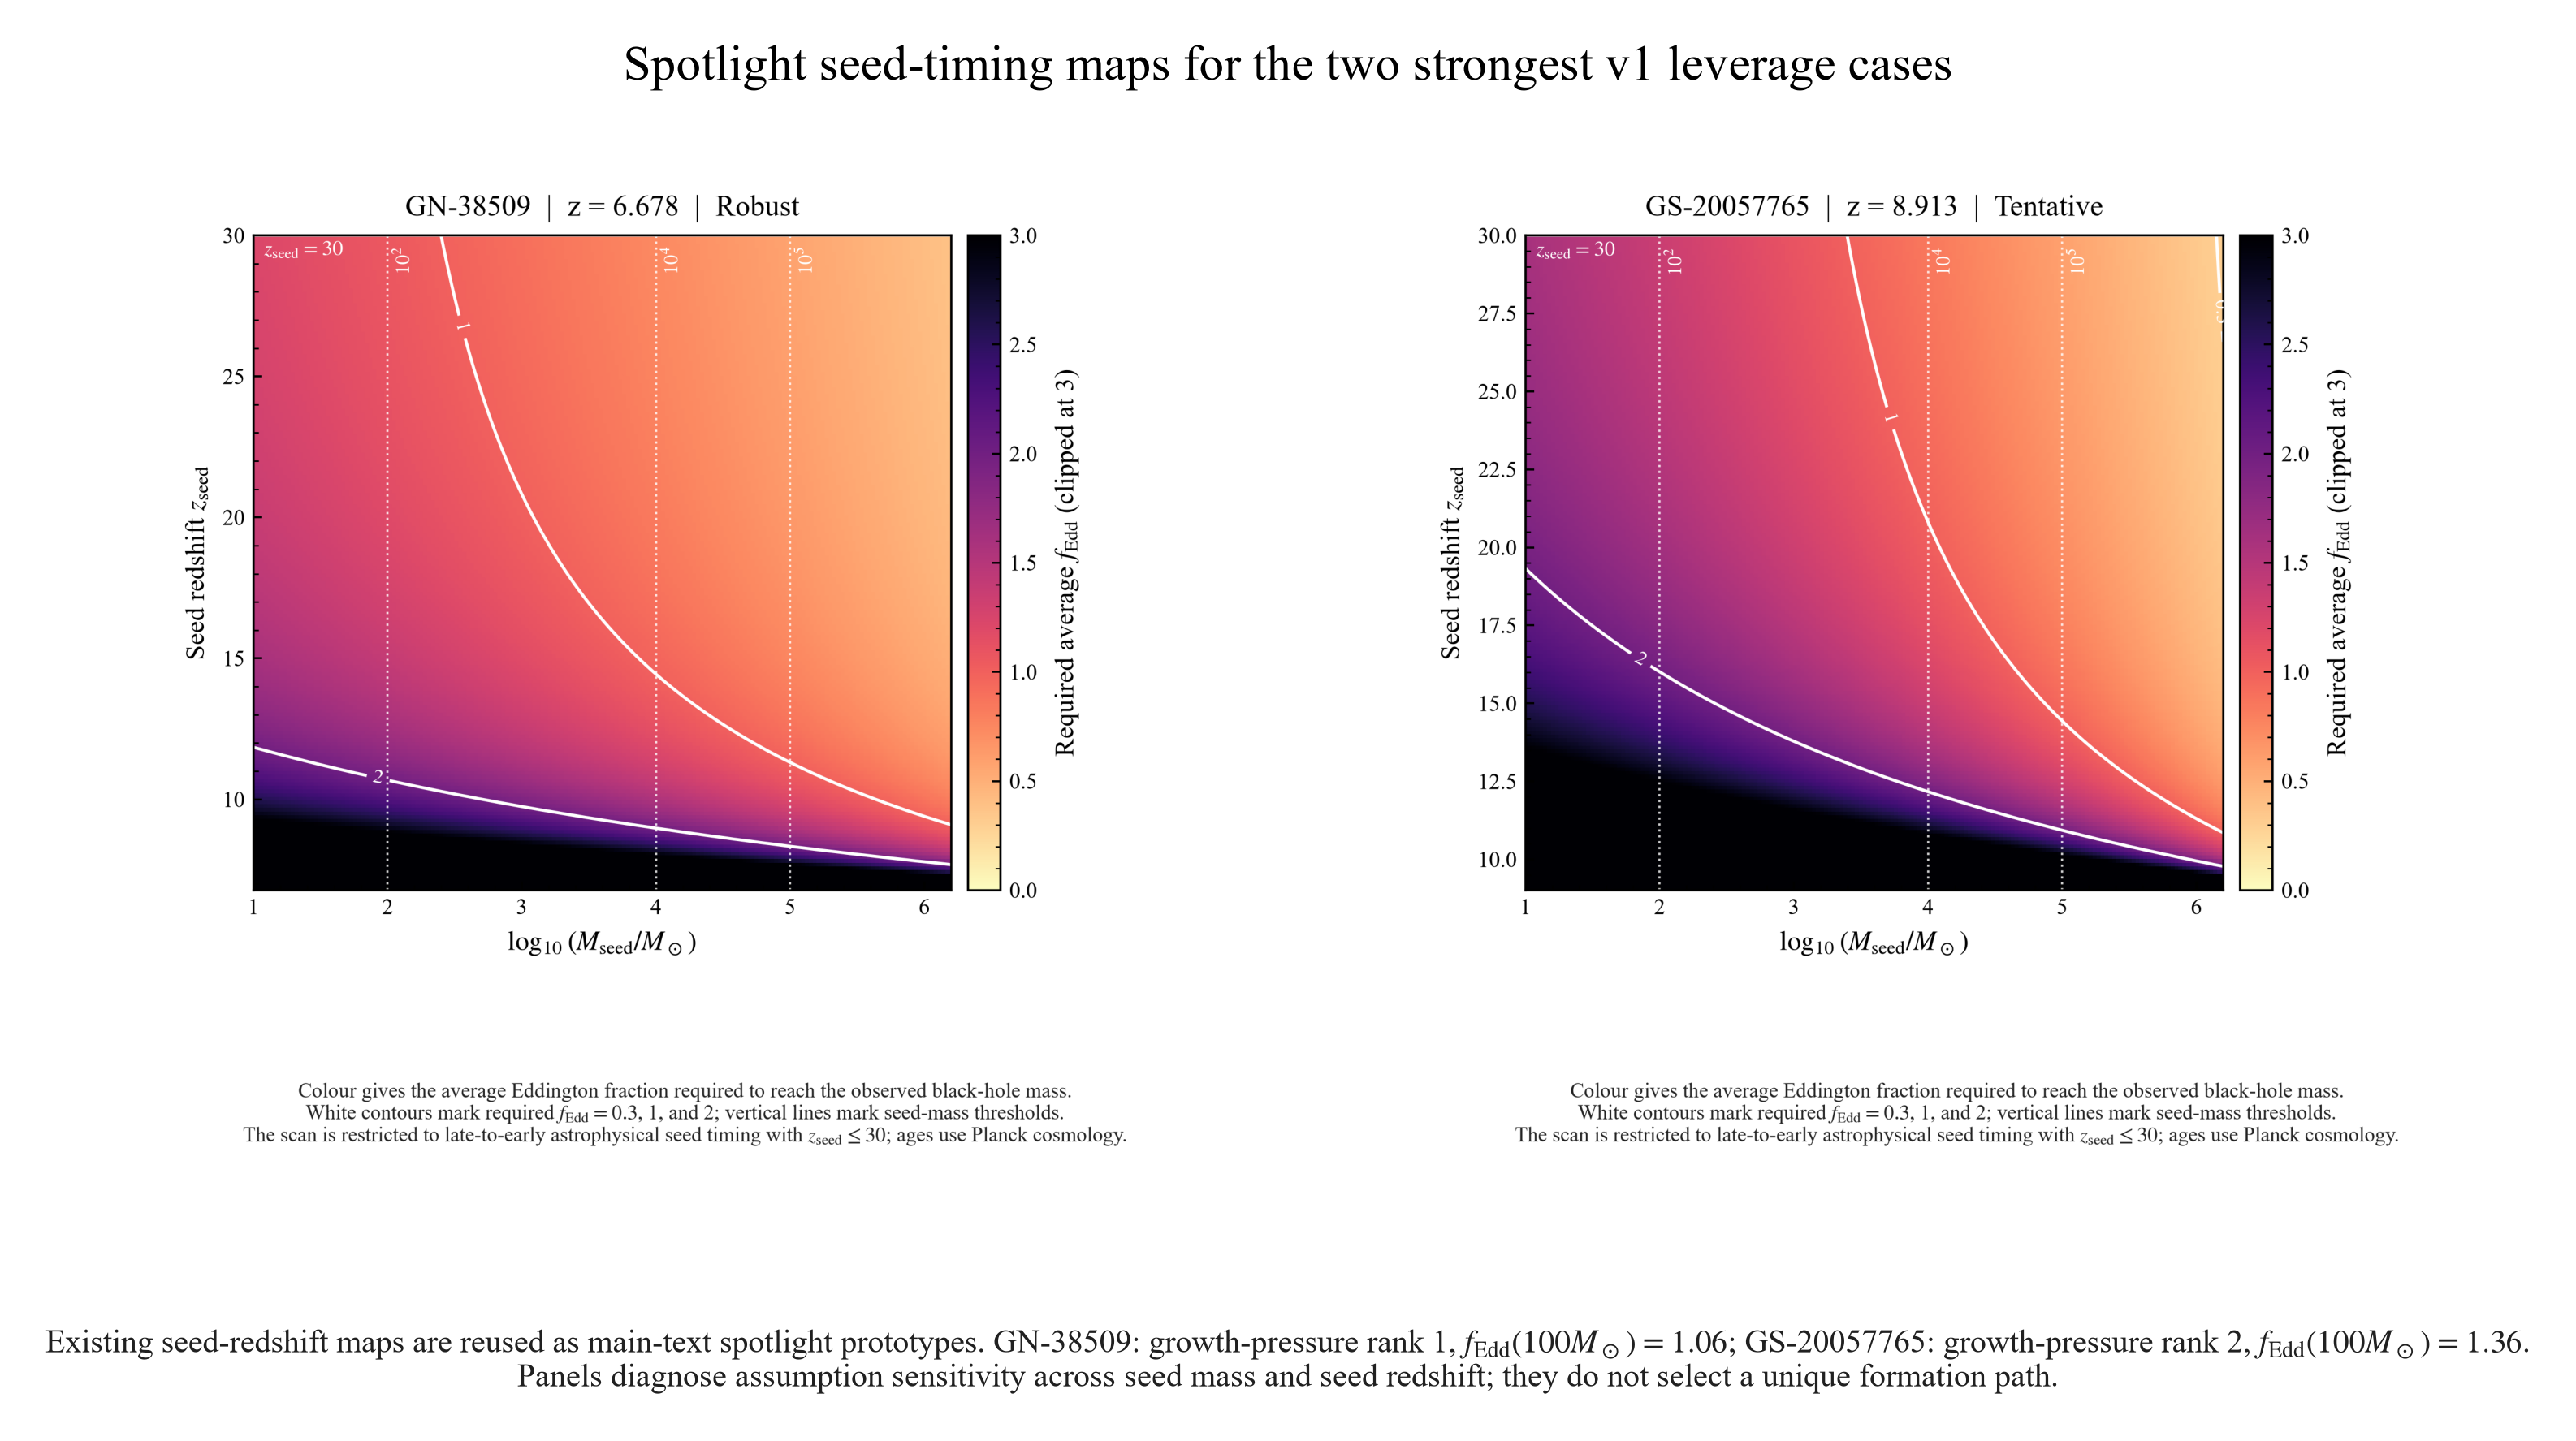
\includegraphics[width=0.98\textwidth]{../results/v2_main_text_figures/v2_main_text_spotlight_seed_redshift_maps.png}
\caption{Seed-redshift spotlight maps for GN-38509 and GS-20057765. These maps show how the required lifetime-average accretion rate changes with seed mass and formation time. The full object gallery is retained for supplementary use; selected panels connect the sample ranking to object-level physical interpretation.}
\label{fig:spotlight}
\end{figure}

\clearpage
\section{Conclusion}

The completed v1--v6 work demonstrates the atlas concept: provenance-aware ingestion, validated standardization, explicit reviewed measurement/object identity, transparent physical modeling, point and Monte Carlo rankings, selection-aware summaries, duplicate-measurement sensitivity, class-aware scaffolding, effective two-state duty-cycle diagnostics, release-specific visualization, and automated regression checks. v6 adds six new THRILS objects while preserving every v1--v5 artifact and default. The full 112/105 ordering remains an exploratory diagnostic, while primary rank claims use the 111/104 evidence-supported population. No THRILS object displaces the established leading primary objects. This is not evidence that one formation pathway is required. The citation/figure audit and class contract are complete; heterogeneous v7 work begins only after a source passes the admission gate.

\begin{thebibliography}{9}
\bibitem{dayal2024}
Dayal, P. 2024, \emph{A\&A}, 690, A182, doi:10.1051/0004-6361/202451481.

\bibitem{juodzbalis2026}
Juod\v{z}balis, I. et al. 2026, ``JADES: comprehensive census of broad-line AGN from Reionization to Cosmic Noon revealed by JWST,'' \emph{MNRAS}, 546, stag086, doi:10.1093/mnras/stag086.

\bibitem{taylor2025}
Taylor, A. J. et al. 2025, ``Broad-Line AGN at $3.5<z<6$: The Black Hole Mass Function and a Connection with Little Red Dots,'' \emph{ApJ}, 986, 165, doi:10.3847/1538-4357/add15b.

\bibitem{matthee2024}
Matthee, J. et al. 2024, ``Little Red Dots: an abundant population of faint AGN at $z\sim5$ revealed by the EIGER and FRESCO JWST surveys,'' \emph{ApJ}, 963, 129, doi:10.3847/1538-4357/ad2345.

\bibitem{lin2024}
Lin, X. et al. 2024, ``ASPIRE: Broad-line AGN at $z=4$--5 revealed by JWST/NIRCam WFSS,'' \emph{ApJ}, 974, 147, doi:10.3847/1538-4357/ad6565.

\bibitem{harikane2023}
Harikane, Y. et al. 2023, ``A JWST/NIRSpec First Census of Broad-Line AGNs at $z=4$--7: Detection of 10 Faint AGNs with $M_{\rm BH}\sim10^6$--$10^8\,M_\odot$ and Their Host Galaxy Properties,'' \emph{ApJ}, 959, 39, doi:10.3847/1538-4357/ad029e.

\bibitem{davis2026}
Davis, K. et al. 2026, ``Extreme Emission Line Galaxies in CEERS Are Powered by Star Formation, not AGN,'' arXiv:2602.23310v1, submitted to \emph{ApJ}.

\bibitem{hutchison2025}
Hutchison, T. A. et al. 2025, ``THRILS -- The High-(Redshift+Ionization) Line Search: Program Description \& Redshift Catalog,'' arXiv:2512.12509v1.
\end{thebibliography}

\end{document}
